\documentclass{tufte-book}

\hypersetup{colorlinks}

\title{Modern Analysis}
\author[The Tufte-LaTeX Developers]{Claire A. Saint-Donat}
\publisher{Columbia University, Fall 2013}
\usepackage{lipsum}


\usepackage{booktabs}
\usepackage{amsmath, amsthm, amssymb}
\usepackage{amsmath}
\usepackage{amssymb}
\usepackage{amsfonts}
\usepackage{url}
\usepackage{xy}
\usepackage{mathrsfs}
\usepackage{hyperref}
\usepackage{verbatim}
\usepackage{enumerate}
\usepackage{multicol}
\usepackage{manfnt}
\usepackage{amsthm}
\usepackage{titletoc}
\usepackage{amssymb}
\usepackage{graphicx}
\setkeys{Gin}{width=\linewidth,totalheight=\textheight,keepaspectratio}
\graphicspath{{graphics/}}


\usepackage{fancyvrb}
\fvset{fontsize=\normalsize}


\setcounter{chapter}{1}
\setcounter{secnumdepth}{2}


\newtheorem{theorem}{Theorem}[chapter]
\newtheorem{lemma}[theorem]{Lemma}
\newtheorem{corollary}[theorem]{Corollary}
\newtheorem{proposition}{Proposition}[chapter]
\theoremstyle{definition}
\newtheorem{definition}{Definition}[chapter]
\newtheorem*{remark}{Remark}
\newtheorem*{example}{Example}
\newtheorem*{imp}{Important point}
\newtheorem*{dangerousbend}{\textdbend Caution}
\newtheorem*{summary}{Summary}
\renewcommand{\thesection}{\thechapter.\arabic{section}}
\numberwithin{section}{chapter}


\newcommand{\hangp}[1]{\makebox[0pt][r]{(}#1\makebox[0pt][l]{)}}

\newcommand{\hangstar}{\makebox[0pt][l]{*}}

\usepackage{xspace}

\newcommand{\vdqi}{\textit{VDQI}\xspace}
\newcommand{\ei}{\textit{EI}\xspace}
\newcommand{\ve}{\textit{VE}\xspace}
\newcommand{\be}{\textit{BE}\xspace}
\newcommand{\VDQI}{\textit{The Visual Display of Quantitative Information}\xspace}
\newcommand{\EI}{\textit{Envisioning Information}\xspace}
\newcommand{\VE}{\textit{Visual Explanations}\xspace}
\newcommand{\BE}{\textit{Beautiful Evidence}\xspace}

\newcommand{\TL}{Tufte-\LaTeX\xspace}

\newcommand{\monthyear}{%
  \ifcase\month\or January\or February\or March\or April\or May\or June\or
  July\or August\or September\or October\or November\or
  December\fi\space\number\year
}


\newcommand{\openepigraph}[2]{%
  %\sffamily\fontsize{14}{16}\selectfont
  \begin{fullwidth}
  \sffamily\large
  \begin{doublespace}
  \noindent\allcaps{#1}\\% epigraph
  \noindent\allcaps{#2}% author
  \end{doublespace}
  \end{fullwidth}
}


\newcommand{\blankpage}{\newpage\hbox{}\thispagestyle{empty}\newpage}

\usepackage{units}

% Typesets the font size, leading, and measure in the form of 10/12x26 pc.
\newcommand{\measure}[3]{#1/#2$\times$\unit[#3]{pc}}

% Macros for typesetting the documentation
\newcommand{\hlred}[1]{\textcolor{Maroon}{#1}}% prints in red
\newcommand{\hangleft}[1]{\makebox[0pt][r]{#1}}
\newcommand{\hairsp}{\hspace{1pt}}% hair space
\newcommand{\hquad}{\hskip0.5em\relax}% half quad space
\newcommand{\TODO}{\textcolor{red}{\bf TODO!}\xspace}
\newcommand{\ie}{\textit{i.\hairsp{}e.}\xspace}
\newcommand{\eg}{\textit{e.\hairsp{}g.}\xspace}
\newcommand{\na}{\quad--}% used in tables for N/A cells
\providecommand{\XeLaTeX}{X\lower.5ex\hbox{\kern-0.15em\reflectbox{E}}\kern-0.1em\LaTeX}
\newcommand{\tXeLaTeX}{\XeLaTeX\index{XeLaTeX@\protect\XeLaTeX}}
% \index{\texttt{\textbackslash xyz}@\hangleft{\texttt{\textbackslash}}\texttt{xyz}}
\newcommand{\tuftebs}{\symbol{'134}}% a backslash in tt type in OT1/T1
\newcommand{\doccmdnoindex}[2][]{\texttt{\tuftebs#2}}% command name -- adds backslash automatically (and doesn't add cmd to the index)
\newcommand{\doccmddef}[2][]{%
  \hlred{\texttt{\tuftebs#2}}\label{cmd:#2}%
  \ifthenelse{\isempty{#1}}%
    {% add the command to the index
      \index{#2 command@\protect\hangleft{\texttt{\tuftebs}}\texttt{#2}}% command name
    }%
    {% add the command and package to the index
      \index{#2 command@\protect\hangleft{\texttt{\tuftebs}}\texttt{#2} (\texttt{#1} package)}% command name
      \index{#1 package@\texttt{#1} package}\index{packages!#1@\texttt{#1}}% package name
    }%
}% command name -- adds backslash automatically
\newcommand{\doccmd}[2][]{%
  \texttt{\tuftebs#2}%
  \ifthenelse{\isempty{#1}}%
    {% add the command to the index
      \index{#2 command@\protect\hangleft{\texttt{\tuftebs}}\texttt{#2}}% command name
    }%
    {% add the command and package to the index
      \index{#2 command@\protect\hangleft{\texttt{\tuftebs}}\texttt{#2} (\texttt{#1} package)}% command name
      \index{#1 package@\texttt{#1} package}\index{packages!#1@\texttt{#1}}% package name
    }%
}% command name -- adds backslash automatically
\newcommand{\docopt}[1]{\ensuremath{\langle}\textrm{\textit{#1}}\ensuremath{\rangle}}% optional command argument
\newcommand{\docarg}[1]{\textrm{\textit{#1}}}% (required) command argument
\newenvironment{docspec}{\begin{quotation}\ttfamily\parskip0pt\parindent0pt\ignorespaces}{\end{quotation}}% command specification environment
\newcommand{\docenv}[1]{\texttt{#1}\index{#1 environment@\texttt{#1} environment}\index{environments!#1@\texttt{#1}}}% environment name
\newcommand{\docenvdef}[1]{\hlred{\texttt{#1}}\label{env:#1}\index{#1 environment@\texttt{#1} environment}\index{environments!#1@\texttt{#1}}}% environment name
\newcommand{\docpkg}[1]{\texttt{#1}\index{#1 package@\texttt{#1} package}\index{packages!#1@\texttt{#1}}}% package name
\newcommand{\doccls}[1]{\texttt{#1}}% document class name
\newcommand{\docclsopt}[1]{\texttt{#1}\index{#1 class option@\texttt{#1} class option}\index{class options!#1@\texttt{#1}}}% document class option name
\newcommand{\docclsoptdef}[1]{\hlred{\texttt{#1}}\label{clsopt:#1}\index{#1 class option@\texttt{#1} class option}\index{class options!#1@\texttt{#1}}}% document class option name defined
\newcommand{\docmsg}[2]{\bigskip\begin{fullwidth}\noindent\ttfamily#1\end{fullwidth}\medskip\par\noindent#2}
\newcommand{\docfilehook}[2]{\texttt{#1}\index{file hooks!#2}\index{#1@\texttt{#1}}}
\newcommand{\doccounter}[1]{\texttt{#1}\index{#1 counter@\texttt{#1} counter}}

% Generates the index
\usepackage{makeidx}
\makeindex

\begin{document}

\frontmatter

\maketitle

\newpage\thispagestyle{empty}
\openepigraph{%
Real mathematics must be justified as art, if it can be justified at all.
}{G.H. Hardy
}
\vfill
\openepigraph{%
The natural numbers are the work of God.  All the rest is the work of mankind.
}{Leopold Kronecker}
\vfill
\openepigraph{%
\ldots It has been our experience that a mathematical question resolved by a counterexample has the pungency of good drama.  Many of the most elegant and artistic contributions to mathematics belong to this genre.
}{Bernard R. Gelbaum}


\vfill
\openepigraph{%
If people do not believe that mathematics is simple, it is only because they do not realize how complicated life is.}{ John von Neumann}

\vfill
\openepigraph{%
God exists since mathematics is consistent, and the Devil exists since we cannot prove it.}{Andr\'{e} Weil}

%\vfill
%\openepigraph{%A mathematician is a person who can find analogies between theorems; a better mathematician is one who can see analogies between proofs and the best mathematician can notice analogies between theories. One can imagine that the ultimate mathematician is one who can see analogies between analogies.}{Stefan Banach}


% r.3 full title page
%\maketitle


% r.5 contents
\tableofcontents

%\listoffigures

%\listoftables

% r.7 dedication
%\cleardoublepage
%~\vfill
%\begin{doublespace}
%\noindent\fontsize{18}{22}\selectfont\itshape
%\nohyphenation
%Dedicated to those who appreciate \LaTeX{} 
%and the work of \mbox{Edward R.~Tufte} 
%and \mbox{Donald E.~Knuth}.
%\end{doublespace}
%\vfill
%\vfill
%
%
%
%\cleardoublepage




%\maketitle

\chapter*{Introduction}
\noindent This document is written in the Tufte handout \LaTeX\ document style.
It provides examples and definitions from Walter Rudin's famous text on Mathematical Analysis which I read in the Fall of 2013 at Columbia University.  What follows are my notes and observations from this critical mathematical work.




\chapter{Chapter One: The Real and Complex Number Systems}\label{sec:page-layout}

In order to have a fruitful discussion on the main concepts of analysis (namely, convergence, continuity, differentiation, and integration) we must first begin with an accurately-defined \textsc{number} concept.

We shall assume all of the axioms that govern arithmetic of the integers and assume familiarity with the rational numbers.  

We will demonstrate how the rational number system is inadequate for many purposes, both as a \textsc{field} and as an \textsc{ordered set}.   (These terms will be defined shortly).   This leads to a natural introduction of the "irrational numbers."

\newthought{The purpose of our discussion of the real numbers}, will be to show that the rational number system has certain gaps, in spite of the fact that between any two rationals there is another. \marginnote{If $r<s$ then $r< \frac{(r+s)}{2} < s$.}  The real number system on the other hand, fills these gaps.  This is the principle reason for the fundamental role it plays in analysis. 

\bigskip

\section{The Axiom of Completeness}
\subsection{Ordered Sets}\label{sec:sidenotes}
%\marginnote{Here are some standard set-theory terms that will be used throughout:  If $A$ is any set (whose elements may be numbers or any other objects), we write $x \in A$ to indicate that $x$ is a member of $A$.   If $x$ is not a member of $A$, we write that $x \notin A$. \\  The set which contains no element will be called the \textsc{empty set}.   If a set has at least one element, it is called nonempty. \\  If $A$ and $B$ are sets, and if every element of $A$ is an element of $B$, we say that $A$ is a subset of $B$ and write $A \subset B$ or $B \supset A$.  If, in addition, there is another element of $B$ not in $A$ then we say that $A$ is a proper subset of $B$.   Note that $A \subset A$ for every set $A$ \\ If $A \subset B$ and $B\subset A$ , we write that $A=B$.  Otherwise $A \neq B$.  }
In order to elucidate the structure of the real numbers as well as that of the complex numbers, we must start with a brief discussion of the general concepts of ordered set and field.



\begin{definition}Let $S$ be a set.  An \textsc{order} on $S$ is a relation, denoted by $<$, with the following two properties

\begin{itemize}
	\item  If $x \in S$ and $y \in S$ then one and only one\footnote{Trichotomy: Between any two elements in the set, only one of the relations can hold.  There is a unique relationship between any two elements.} of the following statements is true:	\[	x< y \qquad x=y \qquad y<x\]  
	\item If $x,y,z \in S$ and, if $x<y$ and $y<z$ then $x<z$
	\footnote{Transitivity}
\end{itemize}
\end{definition}


The statement "$x<y$" may be read as "x is less than y" or "x is smaller than y" or even "x precedes y."

The notation $x \leq y$ indicates that $x<y$ or $x=y$ without specifying which of these two is in fact the case.  In other words $x \leq y$ is the negation of $y<x$.


\begin{definition}An {ordered set} is a set $S$ in which an order is defined.  For example, Q is an ordered set if $r<s$ is defined to mean that $s-r$ is a positive rational number. \end{definition}



\begin{definition}Suppose that $S$ is an ordered set and that $E \subset S$.  If there exists a $\beta \in S$ such that $x \leq \beta$ for every $x \in E$ then we say that $E$ is \textsc{bounded above} and call that $\beta$ an \textsc{upper bound} of $E$.  Lower bounds are similarly defined. \end{definition}


\begin{definition} Suppose that $S$ \marginnote{An alternative and often useful definition of supremum is as follows:  Assume $\alpha \in S$ and is an upper bound for a set $E \subset S$.  Then $\alpha= \sup E$ iff $\forall \quad \varepsilon>0 $ there exists an element $x \in E$ such that $\alpha-\varepsilon < x.$}
is an ordered set, $E \subset S$ and $E$ is bounded above.    Suppose that there exists an $\alpha \in S$ with the following properties:
\begin{itemize}
	\item $\alpha$ is an upper bound of $E$
	\item If $\gamma< \alpha$ then $\gamma$ is not an upper bound of $E$
\end{itemize}
The $\alpha$ is called the \textsc{least upper bound} \footnote{that there is a most one such $\alpha$ is clear from the second premise} or the \textsc{supremum of $E$} and we write
\[\alpha = \sup E\]
\end{definition}

The greatest lower bound of infimum of a set which is bounded below if defined in a similar manner.




\begin{figure}
  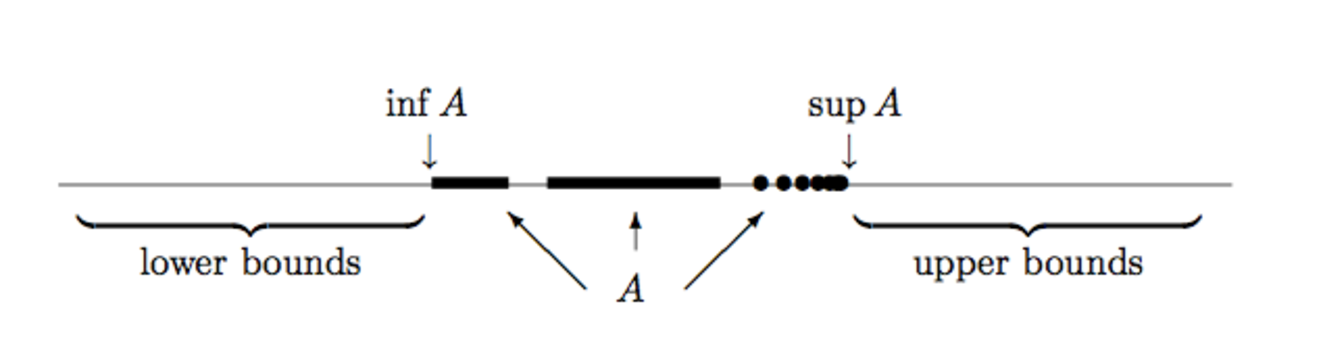
\includegraphics{SupInf.pdf}
%  \checkparity This is an \pageparity\ page.%
  \caption{An example of Supremums and Infimums.}
  %\label{fig:textfig}
  %\zsavepos{pos:textfig}
  \setfloatalignment{b}
\end{figure}

\section{Examples}
Let us now show that $\sqrt{2}$ is irrational.

\begin{proposition} There is no such rational $p$ such that $p^2 = 2$. \end{proposition}

\begin{proof}  If there were such a $p$, we could write $p=m/n$ where $m$ and $n$ are both integers that are not both even (alternatively that $\gcd(m,n) = 1$).  Let us assume this is done.\\
Then we have that $m^2 = 2n^2$.  Hence $m$ is even. \marginnote{$k^2$ is even $\iff$ $k$ is even for all $k \in \mathbb{Z}$}.  Then $m=2k$ for some $k$ and $m^2 = (2k)^2 = 4k^2 = 2n^2$.  Therefore $n^2$ is also even and so therefore is $n$.\\
This conclusion is contrary to our choice of $m$ and $n$.  Hence there exists no such rational $p$. \end{proof}

Let's now examine the situation a little more closely.   Let $A$ be the set of all positive rationals such that $p^2 < 2$ and let $B$ consist of all the positive rationals such that $q^2 > 2$.  We can see that $A$ contains no largest member and $B$ contains no smallest, despite the fact that they are bounded above and below respectively.  Therefore $A$ has no least upper bound in $\mathbb{Q}$ and $B$ has no greatest lower bound in $\mathbb{Q}$.  \\

\newthought{Let $E$} consist of all numbers $1/n$ where $n=1,2,3,\ldots$.  Then, $\sup E = 1 \in E$ and $\inf E =0$ which is not in $E$.  This is to demonstrate that infimum and supremum may or may not be included in the sets which they bound.


\section{Least Upper Bound Property}\label{sec:figures-and-tables}
An ordered set $S$ is said to have the \textsc{least-upper-bound property} is the following is true:

\begin{fullwidth}
If $E \subset S$, $E$ is not empty, and $E$ is bounded above, then $\sup E $ exists in $S$.
\end{fullwidth}

Abbott calls this the Axiom of Completeness and purports that it is the final, most distinctive assumption about the real number system.

For example, we have already shown by a previous example that $\mathbb{Q}$ does not have the least upper bound property.


We shall now show with a central theorem that there is a close relation between greatest lower bounds and least upper bounds, and that every ordered set with the least upper bound property also has the greatest lower bound property.

\begin{theorem} \marginnote{Every ordered set with the least upper bound property, also has the greatest lower bound property.}
Suppose that S is an ordered set with the least-upper bound property, $B \subset S$, $B$ is not empty and $B$ is bounded below.

Let $L$ be the set of all lower bounds of $B$.  Then
\[\alpha = \sup L\]
exists in $S$ and $\alpha = \inf B$.

In particular, $\inf B$ exists in $S$.
\end{theorem}

\begin{proof}
Since $B$ is bounded below, $L$ is not empty.  Since $L$ consists of exactly those $y \in S$ which satisfy the inequality $y \leq x$ for every $x \in B$, we see that every $x \in B$ is an upper bound of $L$.  Thus $L$ is bounded above.  Our hypothesis about $S$ implies therefore that $L$ has a supremum in $S$; call it $\alpha$.

If $\gamma < \alpha$ then $\gamma$ is not an upper bound of $L$, hence $\gamma \notin B$.  It follows that $\alpha \leq x$ for every $x \in B$.  Thus $\alpha \in L$.    

If $\alpha < \beta$ then $\beta \notin L$,  since $\alpha$ is an upper bound of $L$.

We have shown that $\alpha \in L$ but $\beta \notin L$ if $\beta> \alpha$.  In other words, $\alpha$ is a lower bound of $B$, but $\beta$ is not if $\beta>\alpha$.  This means that $\alpha = \inf B$.
\end{proof}

\section{Consequences of Completeness}

Complete metric spaces often have certain nice properties as a result of having least upper bounds.  What follows are some of the consequences of the Completeness Axiom.

For simplicity, we often assume that complete metric space we are working in is the real number line, but be advised that these properties will hold in any metric space with similar properties.

\begin{theorem}\marginnote{Nested Interval Property}  For each $n \in N$ assume we are given a closed interval $I_n = [a_n , b_n] = \{ x \in R : a_n \leq x \leq b_n\}$.  Assume also that each $I_n$ contains $I_{n+1}$.  Then, the resulting sequence of nested intervals, 

\[I_1 \supseteq I_2 \supseteq I_3 \supseteq I_4 \supseteq \cdots \]

has a nonempty intersection; that is, $\cap_{n=1}^{\infty} I_n \neq \emptyset$.
\end{theorem}

\begin{proof}
Knowing that we want to use the AoC to produce a single real value  $x$ satisfying $x \in I_n$ for all $N$, we should consider a bounded set such that its supremum might be this $x$.  Let us consider the set 
\[ A = \{a_n : n \in N\}\]
of the left-handed endpoints of the intervals.

\begin{marginfigure}
  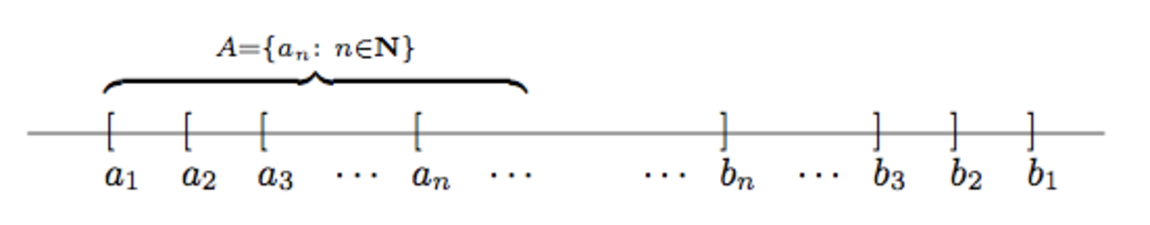
\includegraphics{NIP.pdf}
  \caption{An example of the Nested Interval Property.}
 % \label{fig:textfig}
\end{marginfigure}


Because the intervals are nested, we see that every $b_n$ serves as an upper bound for $A$.  Thus, we are justified in setting
\[ x = \sup A.\]

Now, consider a particular $I_n = [a_n , b_n]$.  Because $x$ is an upper bound for $A$, we have $a_n \leq x$.  The fact that each $b_n$ is an upper bound for $A$ and that $x$ is the least upper bound implies $x\leq b_n$.

Altogether then, we have $a_n \leq x \leq b_n$, which means $x \in I_n$ for every choice of $n \in N$.  Hence, $x \in \cap_{n=1}^{\infty} I_n$ and the intersection is not empty.
\end{proof}


\section{The Density of Q and C in R}
Again here, we are restricting our discussion to the real numbers.  

\begin{theorem}\marginnote{Archimedean Property}  \begin{itemize}[(i)] 
\item  Given any number $x \in R$ there exists an $n \in N$ such that $x<n$.  \item Given any real number $y>0$, there exists an $ n \in N$ such that $\frac{1}{n}< y$. \end{itemize} \end{theorem}

\begin{proof}   Part (i) of the proposition states that N is not bounded above.  This might seem obvious and not in need of a proof yet it is important to note that a set might posses the Archimedean property without being Complete- take Q for example- but a demonstration of this fact requires an investigation into the axiomatic construction of the ordered field in question. In the case of R, the AoC furnishes us with a very short argument.

Assume that N is bounded above.  By the Axiom of Completeness, N should then have a least upper bound property, and we can set $\alpha = \sup N$.  If we were to consider $\alpha -1$, then we no longer have an upper bound and therefore there exists an $n \in N$ such that $\alpha - 1 < n$.  But this is equivalent to $\alpha < n+1$. But because $n+1 \in N$ we have a contradiction to the fact that $\alpha $ is meant to be  an upper bound for $N$.  \marginnote{The contradiction here rests on the AoC and the fact that N is closed under addition.}

For part (ii) just let $x = 1/y$ from above.
Note that $\frac{1}{n} < y$ implies that $\frac{1}{y} < n$.  Therefore this proposition again states that N is not bounded above and the proof is exactly as before.
\end{proof}

\begin{theorem}  \marginnote{Density of C and Q in R}  

\begin{itemize}[(i)] 
\item    For every two real number $a$ and $b$ with $a<b$, there exists a rational number $r$ satisfying $a<r<b$
\item Given any two real numbers $a$ and $b$ with $a<b$. there exists an irrational number $t$ satisfying $a<t<b$
 \end{itemize} \end{theorem}
 
 \begin{proof}
 \begin{itemize}[(i)]
 	\item WLOG assume that  $0 \leq a \leq b$.  A rational number is a quotient, therefore there exists $n,m \in N$ such that 
	\[	a  < \frac{m}{n} < b	\]
 The first step is to choose a denominator large enough so that consecutive increments of size $1/n$ are too close together to "step over" the interval $(a,b)$.
 
 Using the Archimedean property, we pick $n \in N$ so that 
 \[		\frac{1}{n} < b-a\]
The first inequality gives us $na < m <nb$.  With $n$ already chosen, we choose $m$ to be the smallest integer great that $na$.  In other words.
$$m-1 \leq na < m$$ 
which yields $a < m/n$.  The second equality is also equivalent to $a< b - 1/n$ and we can use the third to write,
$$  m \leq na +1$$
$$<  n \big( b - \frac{1}{n} \big) + 1 $$
$$ = nb $$

Because $m<nb$ implies that $m/n < b$, and we have that $a<m/n <b$ as desired.

\item  We want to prove the existence of an irrational number between any two real numbers $a$ and $b$.  Using the density of $Q$ in $R$ on the real number $a - \sqrt{2}$ and $b - \sqrt{2}$ we can find a rational number $r$ such that $a - \sqrt{2} < r < b - \sqrt{2}$.  This then implies that $a< r + \sqrt{2} < b$.  Since an irrational plus a rational is again an irrational (a result proved in the exercises) it follows that $r + \sqrt{2}$ is irrational.

 
 \end{itemize}
 \end{proof}





\section{Fields}
%Include the field axioms
\subsection{The Real Field}

We now state the existence theorem which is the core of this chapter.

\begin{theorem}  \marginnote{Here, we only state the existence of $\mathbb{R}$ but we do not yet provide a proof of its existence.}There exists an ordered field $R$ which has the least-upper bound property.   Moreover, $R$ contains $Q$ as a subfield. \end{theorem}


We omit the proof since it is a little tedious.



\section{Exercises}

\allcaps{1.}  If $r$ is nonzero and rational and $x$ is irrational, show that $rx$ and $r+x$ are also irrational. 

\begin{proof}
	i) Assume that $rx$ is rational for contradiction, where $r$ and $x$ are rational and irrational respectively.  Then assume $r = \frac{a}{b}$
 for some $a,b \in Z$, $b \neq 0$
 \[x \cdot \frac{a}{b} = \frac{c}{d} \leftrightarrow x = \frac{bc}{ad}\]
 contradicting our assumption that $x$ is irrational.
 
 ii) Assume for contradiction that $r+x$ is rational. Therefore $x = (r+x) - r$ is the difference between two rational numbers and therefore is rational itself.  This contradicts our assumption that $x$ is irrational.
 \end{proof}
 
\allcaps{4.}  Let E be a nonempty subset of an ordered set; suppose that $\alpha$ is a lower bound of E and that $\beta$ is an upper bound of E.  Prove that $\alpha \leq \beta$.

\begin{proof}
%Include Proof
\end{proof}


\allcaps{5.}  Let $A$ be a nonempty set of real numbers which is bounded below.  Let $-A$ be the set of all numbers $-x$ where $x$ is in $A$.  Prove that $\inf A = -\sup(-A)$.


\begin{proof}
Using the fact that $R$ is an ordered field with the least upper bound property, we can assume that a nonempty subset $A \subseteq R$ that is bounded below has a greatest lower bound or infimum in $R$.  Call it $\alpha$.

Taking an arbitrary member of this subset $x \in A$, we know that $-x \in -A$ by definition of membership in $-A$.  Furthermore by the definition of infimum, we know that $\alpha \leq x$ for all $x\in A$.  As a consequence of Proposition 1.18 (a) we can deduce that $-\alpha \geq -x$ for all $-x \in -A$.

Using an arbitrary element in $-A$, we have shown that $-\alpha \geq -x$ for all $-x \in -A$ which suggests that $-\alpha$ is an upper bound for $-A$.  

What remains to be shown is that $-\alpha$ is a \emph{least} upper bound.  

Choosing some arbitrary element $\beta < -\alpha$, using again Proposition 1.18 (a), we can be sure that $-\beta > \alpha$.  Since $\alpha $, we already know, is the greatest lower bound of $A$, an element greater than $\alpha$ is not a lower bound but a member of $A$.  By the density of the real numbers, there must exist some element of $x \in A$ such that  $x < -\beta$.  Using yet again Proposition 1.18 (a), there exists some element $-x \in -A$ such that $-x > \beta$.  This states strictly then that $\beta$ \emph{cannot} be an upper bound of $-A$.

Therefore, we have shown that any element LESS than $-\alpha$ cannot be an upper bound for $-A$.  This together with the proof that $-\alpha$ is an upper bound for $-A$ shows that $-\alpha$ is the Supremum of $-A$.


By Proposition 1.14 (d), we can be sure that 
$$ -\sup(-A) = -(-\alpha) = \alpha =  \inf(A) $$
as desired.
\end{proof}



\section{Cardinality \& Countability}
\begin{definition}\textsc{Function:}  Consider two sets $A$ and $B$ and suppose that with each element $x$ of $A$ there is associated, in some manner, an element of $B$, which we denote by $f(x)$.  Then $f$ is said to be a \textsc{function} from $A$ to $B$ (or a mapping of $A$ into $B$).  The set $A$ is called the \textsc{domain} of $f$  (we also say that $f$ is defined on $A$) and the elements $f(x)$ are called the values of $f$. The set of all values of $f$ is called the \textsc{range} of $f$.\end{definition}
\bigskip

\begin{definition}\textsc{Image:}  Let $A$ and $B$ be two sets and let $f$ be a mapping of $A$ into $B$.   If $E \subset A$,  $f(E)$ is defined to be the set of all elements $f(x)$ for $x \in E$.   We call $f(E)$ the \textsc{image} of E under f.  \\In this notation, f(A) is the range of f.  It is clear that $f(A) \subset B$.  \\If $f(A) = B$, then we say that f maps \emph{onto} B.  That is, the function is \textsc{surjective}.\end{definition}
\bigskip


\begin{definition}\textsc{Inverse Image:}  If $E \subset B, f^{-1}(E)$ denotes the set of all $x \in A$ such that $f(x) \in E$.  We call $f^{-1}(E)$ the \textsc{inverse image} of $E$ under $f$.  \\
\marginnote{Alternatively, the concept of 1-1 can be expressed as follows:  $f$ is a 1-1 mapping of A into B provided that $f(x_{1}) \neq f(x_{2})$ whenever $x_{1} \neq x_{2}, x_{1} \in A, x_{2} \in A $}


If $y \in B, f^{-1}(y)$ is the set of all $x\in A$ such that $f(x) = y$.  If for each $y \in B, f^{-1}(y)$ consists of at most one element of $A$, then $f$ is said to be a \emph{1-1 (one-to-one) mapping} of A into B. \end{definition}
\bigskip


\begin{definition}\textsc{Cardinality:}  If there exists a 1-1 mapping of A onto B, we say that A and B can be put into 1-1 correspondence, or that A and B have the same \textsc{cardinal number}, or, briefly that A and B are \emph{equivalent}, and we write that $A \sim B $.  This relation is also an equivalence relation and therefore has the following properties:\marginnote{For two finite set A and B, we have $A \sim B$ iff A and B contain the same number of elements. \\
	For infinite sets, however this is a useful definition since the notion of 1-1 correspondence often maintains its clarity.}
	\begin{itemize}
	\item It is reflexive:  $A \sim A$
	\item It is symmetric:  If $A \sim B$ then $B \sim A$
	\item It is transitive:  If $A \sim B$ and $B\sim C$ then $A \sim C$
\end{itemize}\end{definition}
\bigskip


\begin{definition}\textsc{Countability:}  For a set A
\begin{itemize}
	\item A is \textsc{finite} if $A\sim [n]$ for some n \marginnote{Note: the empty set is also considered finite! \quad $A$ is infinite if $A$ is equivalent to one of its proper subsets.}
	\item A is \textsc{infinite} if $A$ is not finite
	\item A is \textsc{countable} if $A \sim N$
	\item A is \textsc{uncountable} if A is neither finite nor countable
	\item A is \textsc{at most countable} if A is either finite or countable
	
\end{itemize}\end{definition}

Notice that $\mathbb{Z}$ is countable.  (We demonstrate this by defining the bijection). 
\marginnote{An example of a 1-1 function from $N \to Z$:
\begin{displaymath}
   f(x) = \left\{
     \begin{array}{lr}
       (n-1)/2 & : n \quad \text{is odd}\\
       -n/2 & : n \quad \text{is even}
     \end{array}
   \right.
\end{displaymath}} 
Also notice that $\mathbb{Q}$ is countable. (We demonstrate this using the Cantor construction).  Likewise, the set of even natural numbers is countable.  We can show this by inventing an appropriate function.


Also notice,  the function $f(x) = \frac{x}{x^2 - 1}$ takes the interval $(-1,1)$ onto $R$ in a 1-1 fashion.   Thus $(-1,1) \sim R$.   In fact, $(a,b) \sim R$ for any interval $(a,b)$.      Therefore, intervals on the real line are uncountable.



A finite set cannot be equivalent to one of its proper subsets.   That is, however possible for infinite sets.  In fact we could replace the definition for infinite with this statement:  A is infinite if A is equivalent to one of its proper subsets.
\bigskip


\noindent \begin{definition}\textsc{Sequence:} \marginnote{Simply put, a sequence is a function whose domain is $\mathbb{N}$} \end{definition}By a sequence, we mean a function $f$ defined on the set of natural numbers.   If $f(n) = x_{n}$ for $n \in \mathbb{N}$, it is customary to denote the sequence f by the symbol $\{x_{n}\}$, or sometimes by $x_{1}, x_{2}, \ldots$. The values of $f$, that is, the elements of the sequence are called terms.  If $A$ is a set and if $x_{n} \in A$ for all $n \in J$, then $\{x_{n}\}$ is said to be a sequence in A, or a sequence of elements of A.\\

Note that the terms of a sequence need not be distinct.\\


\smallskip
Since every countable set is the range of a bijection defined on the set of natural numbers, we can regard every countable set as the range of a sequence of distinct terms.  In other words, the elements of a countable set can be "arranged in a sequence."


\smallskip

\begin{theorem}  If $A$ is countable and $E \subset A$ then $E$ is at most countable, that is finite or countable.  \marginnote{Alternatively, Every infinite subset of a countable set is countable} \end{theorem}

\begin{proof}
Let $E \subset A$.
\indent If $E$ is finite, then we are done. \\
\indent On the other hand assume that $E$ is infinite.  Then let $A = \{x_{1}, x_{2}, \ldots\}$ which we can do since A is countable.  Then we construct a sequence $\{n_{k}\}$ as follows:  Let $n_{1}$ be the smallest natural number such that $x_{n_{1}} \in E$.   Having chosen, $n_{1}, \ldots, n_{k-1}$, let $n_{k}$ be the smallest natural number greater than $n_{k-1}$ such that $x_{n_{k}} \in E$.   Then set $f(k) = x_{n_{k}} \in E$.  This function is a bijection by construction and therefore $E$ is countable.

\end{proof}

This theorem shows that roughly speaking, no uncountable set can be a subset of a countable set.

\begin{theorem}  The union of countably many countable sets is countable.   Let $\{E_{n}\} ,  n=1,2,3,\ldots$ be a sequence of countable sets.  Then the set $S$,
\[S = \bigcup_{n=1}^{\infty} E_{n} \] is countable. \end{theorem}

\begin{proof}
Let every set $E_{n}$ be arranged in a sequence $\{x_{n_k}\}, k = 1,2,3, \ldots$ and consider the infinite array in which the elements of $E_n$ form the nth row of the array.  The array contains all of the elements of $S$.  As in the Cantor construction, these elements can be arranged in a sequence (denoted by the arrows) of the form  
\begin{marginfigure}
  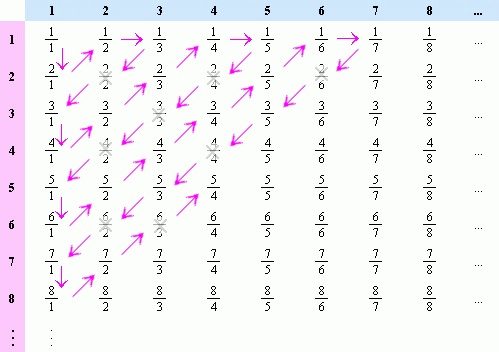
\includegraphics{rationals-countable.jpg}
  \caption{An example of the Cantor Construction for countability proofs.}
 % \label{fig:textfig}
\end{marginfigure}

\[x_{11}; x_{21}, x_{12}; x_{31}, x_{22}, x_{13}; x_{41}, x_{32}, x_{23}, x_{14}; \ldots\]

If any two sets have an element in common these will appear twice in the about sequence.  Therefore there is a subset of the natural numbers, call it T, such that $S \sim T$ which shows that S is at most countable.

However, since $E_{1}\subset S$ and $E_{1}$ is infinite, then S is infinite and thus countable.
\end{proof}

\begin{corollary} Suppose $A$ is at most countable and that for every $\alpha \in A$, there is associated a set $B_{\alpha}$ that is at most countable.  Then the set T
\[T = \bigcup_{\alpha \in A} B_{\alpha}\]
is at most countable. \end{corollary}



\begin{theorem}  A \emph{finite} product of countable sets is countable.  For any n,  $E_{1} \times E_{2} \times \ldots \times E_{n}$ is countable for $E_{i}$ all countable. \end{theorem}

\marginnote{Note that the fact that the product is \emph{finite} is key.  \\Take for example, \\$E = \{0,1\},\quad E \times E \times E \times E \ldots$ \\which is not countable.  (Exercise!)}


\begin{proof}
We complete this proof by induction on n.  For $n=1$, the assertion holds trivially.  Suppose that $E_{1} \times E_{2} \times \ldots \times E_{n-1}$ is countable.  To show this for $E_{1} \times E_{2} \times \ldots E_{n-1}\times E_{n}$, we notice that since $E_{n}$ is countable, we can list its elements as a sequence;  $E_{n}= {y_1, y_2, \ldots}$.  Then

\[E_{1} \times E_{2} \times \ldots E_{n-1}\times E_{n} = \]
\[  \big( E_{1} \times \ldots \times E_{n-1} \times \{y_1\} \big) \cup  \big( E_{1} \times  \ldots \times E_{n-1} \times \{y_2\}\big) \cup  \ldots   \] 

\center{And}
\[E_{1} \times E_{2} \times \ldots E_{n-1}\times E_{n} = \bigcup_{i=1}^{\infty} (E_{1} \times  \ldots \times E_{n-1}) \times \{y_i\}  \] 

Therefore,  $E_{1} \times E_{2} \times \ldots E_{n-1}\times E_{n} $ is equivalent to the countable union of countable sets and, by the theorem above, is also countable.
\end{proof}


\begin{corollary}The set of all rational numbers is countable. \end{corollary}

By the Theorem above, we take $n=2$ noting that every rational is of the form $b/a$ where $a$ and $b$ are both integers.  The set of pairs $(a,b)$ and therefore the set of fractions $b/a$ is countable.  
\medskip

In fact, even the set of all algebraic numbers is countable.

\begin{corollary} 
A complex number is said to be \emph{algebraic} if there are integers $a_{0}, \ldots, a_{n}$ not all zero such that 
$$ a_{0}z^n + a_{1}z^{n-1} + \cdots + a_{n-1}z + a_{n} = 0. $$

Prove that the set of algebraic numbers is countable.
\end{corollary}
 
\begin{proof} 
For each fixed integer $n \geq 0$, let us call the set $P_{n}$ the set of all polynomials with integer coefficients and degree of at most $n$.  We can be sure that such a set is countable since it is equivalent to set of all $n+1$-tuples $(a_{0}, \ldots, a_{n})$, where $a_{i} \in Z$ which is countable, as stated in Theorem 2.13.  

The set of ALL polynomials of every degree with integer coefficients can therefore be expressed as
$$   P = \bigcup^{\infty}_{n=0} P_{n} \qquad \text{where} \ n \in N.$$


By Theorem 2.12, the countable union of countable sets is also countable and therefore P, the set of all polynomials with integer coefficients, is countable.

By the Fundamental Theorem of Algebra, each polynomial of degree $n$ has only finitely many roots (at most $n$). Therefore the set of all possible roots of all polynomials with integer coefficients is a countable union of finite sets, hence countable.
\end{proof}


But note that not all infinite sets are countable as shown in the next theorem.

\begin{theorem} Let A be the set of sequences whose elements are 0's and 1's.  This set A is uncountable. \end{theorem}

\begin{proof}
Let $E$ be a countable subset of A and let E consists of the sequences $s_1, s_2, s_3, \ldots$.   We construct a sequence $s$ as follows: If the nth digit in $s_n$ is 1, we let the nth digit of $s$ be 0, and vice versa.  Then the sequence s differs from every member of E in at least one place and hence, $s \notin E$.  Clearly $s \in A$ however so that E is a proper subset of A.\\

We have shown that every countable subset of A is a proper subset of A.  It follow that A is uncountable (otherwise A would be a proper subset of A which is absurd).
\end{proof}

\begin{proof} \marginnote{Alternative proof presented by Andre}

We proceed to prove by contradiction.  Say A is countable and we can list its elements in an array:  $A = \{x_1, x_2, \ldots \}$.  Let $y = (y_1, y_2, y_3, \ldots)$ be the sequence of 0's and 1's listed along the diagonal in the array.   Define the sequence $z \in A$ as the sequence that exchanges all of the 1's in y for 0's and vice versa.  But then we have that z differs from every $x_i \in A$ in at least one place and hence $z$ cannot be in $A$.  Contradiction.

\end{proof}

\begin{theorem} The open interval $(0,1) \subset \mathbb{R}$ is uncountable.  \marginnote{This theorem is equivalent to the one below and to the theorem which states that R is uncountable.  (0,1) is uncountable iff [0,1] is uncountable iff R is uncountable.  See why this is true.}  \end{theorem}


\begin{proof}
We proceed to prove by contradiction.  Assume that there exists a function $f: \mathbb{N} \to (0,1)$ that is bijective.  Then for each $m \in \mathbb{N}$, $f(m)$ is a real number between 0 and 1, and we represent it using decimal notation

\[f(m) = .a_{m1}a_{m2}a_{m3}a_{m4}a_{m5} \ldots\]


\marginnote{This theorem can also be proved by the production of a bijection from $R \to (0,1)$.  Take for example $$ f(x) = \frac{(x - 1/2)}{(x-x^2)} $$  Since $R$ is uncountable, it must follow that $(0,1)$ is also uncountable.}
What is meant here is that for each $m,n \in \mathbb{N}, a_{mn}$ is the digit from the set $\{0,1,2, \ldots, 9\}$ that represents the nth digit in the decimal expansion of $f(m)$.  Therefore we can index the array of $f(m)'s$ by the digits of their decimal expansion.   We assume that \emph{every} real number between 0 and 1 appears somewhere on this list.\\

Now for the pearl of the argument.   Define a real number $x \in (0,1)$  with the decimal expansion $x=.b_1 b_2 b_3 b_4 \ldots$ using an arbitrary rule such as 

 \begin{displaymath}
   f(x) = \left\{
     \begin{array}{lr}
       2 & : a_{nn} \neq 2 \\
       3 & : a_{nn} = 2
     \end{array}
   \right.
 \end{displaymath} 
   
   
   Since, by construction, this real number x differs from every other number listed, x cannot be a member of $A$ as defined.  Therefore, we have a contradiction.
   
\end{proof}

\begin{theorem} The closed interval $[0,1] \subset \mathbb{R}$ is uncountable.  \end{theorem}
\marginnote{Note that this is true iff R is uncountable.  Also note that this theorem is equivalent to the one below.  From this we can conclude that R is uncountable.}  (Hint: express $x \in [0,1]$ in binary notation)   From this conclusion, we can determine that $\mathbb{R}$ is uncountable.  


\begin{theorem}  (i) The set $\mathbb{Q}$ is countable\\ (ii) The set $\mathbb{R}$ is uncountable.  \marginnote{There are 2 proofs for the countability of $Q$.  \begin{itemize}
\item Function using the Cantor Construction  \item $Q = N \times N$ and is a finite product of countable sets. Therefore countable. \end{itemize}}  \marginnote{There are 4 proofs for the uncountability of $R$:
\begin{itemize}
	\item NIP
	\item Using the binary representations of real numbers and the fact that the sequences of $0s$ and $1s$ is uncountable
	\item There are infinite subsets of $R$ (namely $(0,1)$ and $[1,1]$ ) that are uncountable.
	\item Max Lipyanskiy's Senior Thesis at Columbia
\end{itemize}}
\end{theorem}

\begin{proof}
(i) For each $n \in \mathbb{N}$, let $A_n$ ne the set given by:
\[A_n = \{\pm \frac{p}{q}: \text{where} \quad p,q \in \mathbb{N} \}\]
Also note that we stipulate that p and q are in the lowest possible terms with $p+q=n$.  \\
What's crucial to observe is that every $A_n$ is \emph{finite} and every rational number appears in exactly one of these sets.  Our 1-1 correspondence with the natural numbers is then achieved by listing each of the elements of Q.  \\
(ii) We proceed with a proof by contradiction.  Assume that there exists a bijection $f: \mathbb{N} \to \mathbb{R}$. This suggests that is it possible to enumerate the elements of $\mathbb{R}$.  We can write
\begin{equation}\mathbb{R} = \{x_1, x_2, x_3, x_4, \ldots\}\end{equation}
and be confident that every real number appears somewhere on the list.  We now use something called the Nested Interval Property\marginnote{Nested Interval Property: For each $n \in \mathbb{N}$, assume we are given a closed interval $[a_n, b_n] = \{x \in \mathbb{R}: a_n \leq x \leq b_n\}$.  Assume also that for each $I_n \supset I_{n+1}$.  Then the resulting nested sequence of closed intervals has a nonempty intersection. } to produce a real number that is not there on our list.\\  Let $I_1$ be a closed interval that \emph{does not} contain $x_1$.  Next, let $I_2$ be a closed interval, contained in $I_1$ such that $x_2 \notin I_2$.  The existence of $I_2$ is easy to verify.  Certainly, $I_1$ contains two smaller \emph{disjoint} closed intervals and $x_2$ can only be in one of these.  In general, given an interval $I_n$, construct $I_n+1$ to satisfy \begin{enumerate}
	\item $I_n+1 \subset I_n$ and
	\item $x_{n+1} \notin I_{n+1}$
\end{enumerate}


We now consider the intersection \[ \bigcap_{n=1}^{\infty}I_n \]  

\begin{marginfigure}
  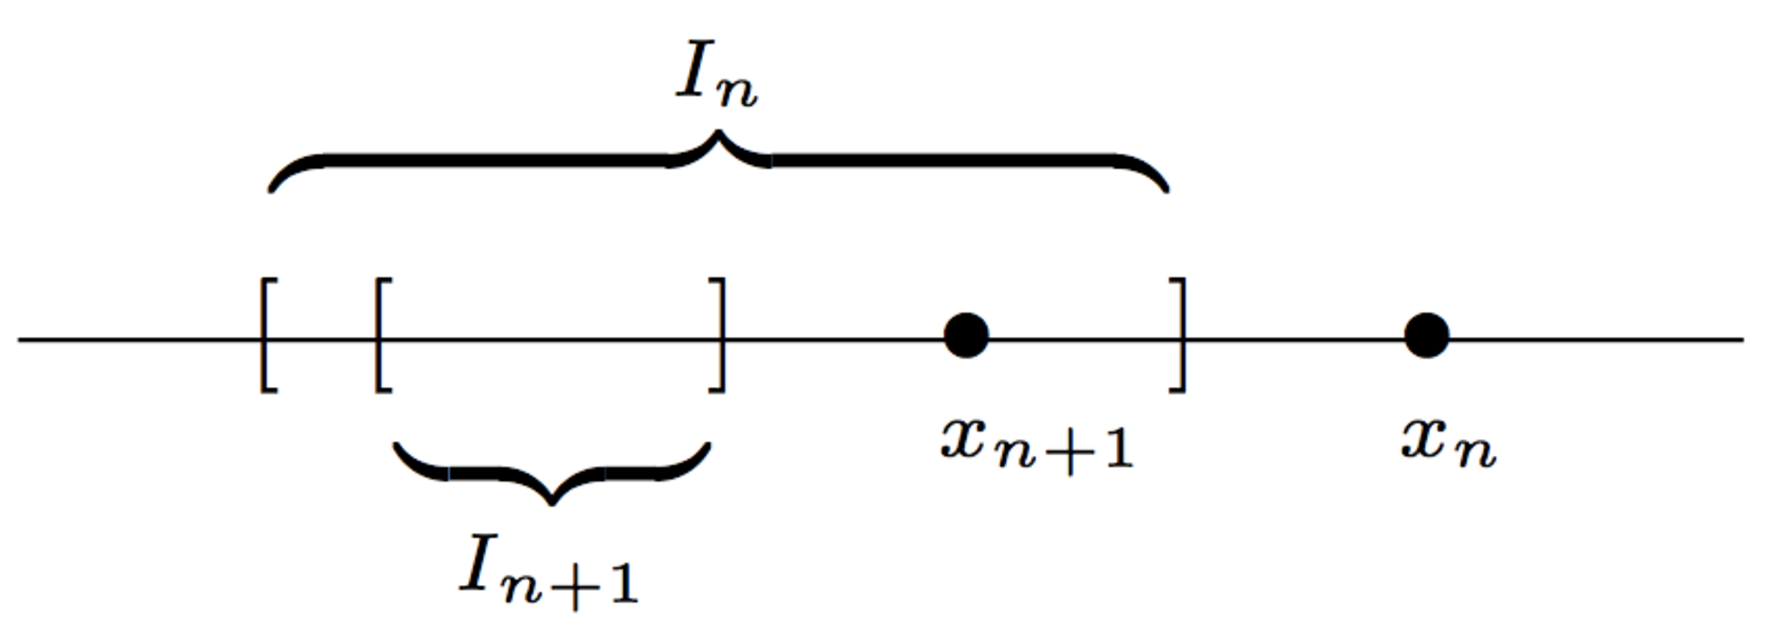
\includegraphics{NIP_RealsUncount.pdf}
 % \label{fig:textfig}
\end{marginfigure}

If $x_{n_0}$ is some real number from the list (1), then we have that $x_{n_0} \notin I_{n_0}$ and therefore not in the intersection of the intervals.\\  Now assuming that (1) contains every real number, this leads to the conclusion that 
\[ \bigcap_{n=1}^{\infty}I_n = \emptyset \]

However, according to the Nested Interval Property this is impossible.  By NIP there is a least one x in the intersection that consequently cannot be on the list in (1).  This contradiction means that such an enumeration of $\mathbb{R}$ is impossible and we can conclude that $\mathbb{R}$ is uncountable.



\end{proof}

\section{Properties of Norms}


Suppose that $\mathbf{x,y,z} \in R^k$ and $\alpha$ is real. Then
\begin{itemize}[$\diamond$]
	\item $|\mathbf{x}| \geq 0$
	\item $|\mathbf{x}| = 0$ iff $\mathbf{x} = 0$
	\item $|\alpha \mathbf{x}| = |\alpha||\mathbf{x}|$
	\item $|\mathbf{x} \cdot \mathbf{y}| \leq |\mathbf{x}| |\mathbf{y}| $
	\marginnote{The Cauchy-Schwarz Inequality}
	\item $|\mathbf{x+y}| \leq |\mathbf{x}|  + |\mathbf{y}|$
	\marginnote{The Triangle Inequality}
	\item $|\mathbf{x}- \mathbf{z}| \leq |\mathbf{x-y}| + |\mathbf{y-z}|$     
\end{itemize}



\setcounter{chapter}{2}
\chapter{Chapter Two: Sequences and Series}


\setcounter{section}{0}
\setcounter{theorem}{0}
\setcounter{definition}{0}
\section{Sequences}

Most of the concepts in analysis can be reduced to statements about the behavior of sequences.  Therefore it is important to have a clear understanding of them before moving forward.




\begin{definition}\textsc{Sequences} are functions whose domain is N.  \end{definition}

The formal definition leads immediately to the familiar depiction of a sequence as an ordered list of real numbers.  Given a function $f: N \to R$,   $f(n)$ is just the nth term on the list.  The notations for sequences reinforce this understanding.

What is crucial to understand is that a sequence is an \emph{infinite} list of real numbers.  What happens at the beginning is of little importance since the business of analysis is concerned with the behavior of the infinite tail of a given sequence.  

\begin{definition}Convergence of a Sequence:  A sequence $(p_n)$ converges to a real number $p$ if, \marginnote{It might be well to point out that our definition of convergent sequence depends not only on the sequence in question but also on the metric space X.}for every positive number $\varepsilon$, there exists an $N \in \mathbb{N}$ such that whenever $n \geq N$ it follows that $|p_n - p|< \varepsilon$. \end{definition}


For Rudin, a sequence $\{p_n\}$ in a metric space X is said to converge if there is a point $p \in X$ with the following property:  For every $\varepsilon > 0$ there is an integer $N$ such that $n \geq N$ implies that $d(p_n, p) < \varepsilon$.

In this case, we also say that  $\{p_n\}$ converges to $p$, or that $p$ is the limit of  $\{p_n\}$ and we write that 
\[\lim_{x \to \infty} \{p_n\} = p   \qquad (p_n) \to p\]


If a sequence does not converge, it is said to diverge.  \marginnote{Note: the definition of divergence depends on the negation of quantifiers.  ie.  There exists an $\varepsilon>0$ such that there is no N where $n\leq N$ implies that $d(p_n, p) < \varepsilon$.}

\begin{definition}
We recall that the set of all points $p_n  (n=1,2,3, \ldots)$  is the \textsc{range} of the sequence.  The range can be infinite or finite.  


 The sequence $\{p_n\}$ is said to be \textsc{bounded} if its range is bounded.  That is, a sequence is bounded if there exists an $M > 0$ such that $|x_n|\leq M$ for all $n \in \mathbb{N}$.\end{definition}


\bigskip
In an effort to decipher this complicated definition, it helps to consider the phrase "$d(p_n, p) < \varepsilon$" and think about the points that satisfy an inequality of this type.


\begin{definition}$\varepsilon-$neighborhoods:  Given a point $p \in X$ and a positive number $\varepsilon > 0$,  the set
\[V_{\varepsilon}(p) = \{x \in X: d(x,p)< \varepsilon\}\]
is called the $\varepsilon-$neighborhood of p. \end{definition}

Notice that $V_{\varepsilon}(p)$ consists of all those points whose distance from p is less than $\varepsilon$.  Recasting the definition of convergence in terms of $\varepsilon-$neighborhoods gives us a more geometric impression of what is being described.

\begin{definition}\newthought{Convergence of a Sequence (Topological Version):}  a sequence $\{p_n\}$ in a metric space X converges to $p$, if, given any $\varepsilon-$neighborhood  $V_{\varepsilon}(p)$ of $p$, there exists a point in the sequence after which all the terms are in $V_{\varepsilon}(p)$.  In other words, every $\varepsilon-$neighborhood centered at $p$ contains all but a finite number of the terms of $\{p_n\}$.
\end{definition}

Notice that these two definitions of convergence say exactly the same thing.  The natural number N from before, is the point where the sequence enters $V_{\varepsilon}(p)$ and never leaves.  It should be apparent that \emph{the value of N depends on the choice of} $\varepsilon$.   

The smaller the $\varepsilon-$neighborhood, the larger N may have to be.


\noindent \emph{Example:}  We claim that $$ \lim \bigg( \frac{1}{\sqrt{n}} \bigg) = 0 $$

\begin{proof}
Let $\varepsilon >0$ be an arbitrary positive number.  Choose a natural number $N$ such that 

$$	\frac{1}{\sqrt{N}} < \varepsilon \implies N > \frac{1}{{\varepsilon}^2}	$$

We now verify that this choice of N has the desired property.  Let $n \geq N$.  Then,

$$	n> \frac{1}{\varepsilon^2}	  \quad \text{implies} \quad \frac{1}{\sqrt{n}} < \varepsilon \quad \text{and hence} \quad |a_{n} -0|< \varepsilon$$

\end{proof}

\section{Some Examples:}

\begin{enumerate}
	\item If $s_n = 1/n$ then $\lim_{n \to \infty} \{s_n\} = 0$.  The range is infinite and the sequence is bounded.
	\item If $s_n = n^2$ then the sequence is divergent, unbounded and has infinite range.
	\item If $s_n = 1 + [{(-1)^n}/n]$ then the sequence $\{s_n\}$ converges to 1, is bounded, and has infinite range.
	\item If $s_n = i^n$, then the sequence is divergent, is bounded, and has finite range.
	\item If $s_n = 1$ then the sequence converges to 1, is bounded, and has finite range.
	\item  Now take the sequence $\{a_n\}= 1/\sqrt{n}$.
	
	Our intuitive understanding tells us that the sequence converges to 0 but let's first explore the relationship between $\varepsilon$ and N in the definition of convergence.
	
	Let's define a sort of "target zone"  and say that we take $\varepsilon = 1/10$.  By claiming that the limit of the sequence is 0, we are saying that the terms of the sequence eventually get arbitrarily close to 0.  
	
	We have set $\varepsilon = 1/10$ as our standard of "closeness" which leads to the neighborhood (-1/10, 1/10) around the limit 0.  How far out into the sequence before the terms fall into this interval?  The 100th term $s_{100} = 1/10$ puts us right on the boundary so we can say that,  if $n>100$ then $s_n \in (-1/10, 1/10)$.  Thus for $\varepsilon = 1/10$ we choose $N=101$ (or anything larger) as our response.
	
	But our choice of $\varepsilon $ was maybe rather whimsical.  How can we assure that for every choice of $\varepsilon $, we can find an appropriate N.  For this problem, the desired relationship is implicit in the algebra carried out to compute our previous answer.  Whatever $\varepsilon $ happens to be, we want 
	\[\frac{1}{\sqrt{n}} < \varepsilon\]
	which is equivalent to 
	\[n > \frac{1}{\varepsilon ^ 2}\]
	
	Now we are ready to write a formal argument.

We claim that \[\lim_{n \to \infty} \{\frac{1}{\sqrt{n}}\} = 0\]

\begin{proof}
Let $\varepsilon> 0 $ be an arbitrary positive number.  Choose the natural number N satisfying $N > \frac{1}{\varepsilon ^ 2}$.  

We now verify that this choice of N has the desired property.  Let $n \geq N$.  Then,
\[n > \frac{1}{\varepsilon^2} \implies \frac{1}{\sqrt{n}}< \varepsilon\]

Then \[|\frac{1}{\sqrt{n}} - 0| < \varepsilon \]  \end{proof}
\end{enumerate}



The  definition of convergence given earlier is the result of hundreds of years of refining the intuitive notion of a limit into a mathematically rigorous statement.  The logic of such a statement is intimately tied to the use of the quantifiers "for all" and "there exists."  The ability to write proofs of convergence depends heavily on a firm understanding of how to manipulate such statements.

\newthought{Template for Proof that $(x_{n}) \to x_{n}$}
	\begin{enumerate}
			\item Let $\varepsilon>0$ be arbitrary
			\item  Demonstrate a choice for $N \in \mathbb{N}$.  This usually requires the most work, which should be done before actually writing the proof (less messy)
			\item Now, show that N actually works
				\begin{enumerate}
						\item Assume $n \geq N$
						\item With $N$ well chosen, it should be possible to derive the inequality that $|x_{n} - x| < \varepsilon$.
				\end{enumerate}
	\end{enumerate}


\noindent \emph{Example:}  We claim that $$ \lim \bigg( \frac{n+1}{n} \bigg) = 1 $$

\begin{proof}
Let $\varepsilon >0$ be an arbitrary positive number.  Choose a natural number $N$ such that $ N > \frac{1}{\varepsilon}	$.


We now verify that this choice of N is appropriate.  Let $n \geq N$.  Then,

$$	n> \frac{1}{\varepsilon}	  \quad \text{implies} \quad \frac{1}{n} < \varepsilon \quad \text{and hence} \quad \bigg|  \frac{n+1}{n}  -1  \bigg|  = \bigg|  \frac{1}{n} \bigg|< \varepsilon$$

as desired.
\end{proof}



Significant insight into the role of the quantifiers in the definition of convergence
can be gained by studying an example of a sequence that does not have a limit.

\begin{definition}Divergence:  A sequence that does not converge is said to diverge. \end{definition}


To prove that a particular number $x$ is not the limit of a sequence $(x_{n})$ we must produce a single value of $\varepsilon$ for which no $N \in \mathbb{N}$ works.
\medskip

\noindent
\emph{Exercise 2.2.1.} Verify, using the definition of convergence of a sequence, that
the following sequences converge to the proposed limit.
\begin{enumerate}[(a)]
\item $\lim \frac{1}{(6n^{2}+1)} = 0$.
\item $\lim \frac{(3n+1)}{(2n+5)} = \frac{3}{2}$.
\item $\lim \frac{ 2}{\sqrt{n+3}} = 0$.
\end{enumerate}

\begin{proof}
	\begin{enumerate}[(a)]
			\item Let $\varepsilon > 0$ be arbitrary. We must show that there exists an
$N \in \mathbb{N}$ such that $n\geq N$ implies $\big|\frac{1}{(6n^{2}+1)} - 0 \big|  < \varepsilon$.  Well, manipulation of the statement tells us that 

$$\bigg|\frac{1}{(6n^{2}+1)} \bigg|  = \frac{1}{(6n^{2}+1)}  \quad \text{and therefore that}$$

$$ \frac{1}{(6N^{2}+1)}  < \varepsilon \quad \text{which implies that} \quad N > \sqrt{\frac{1- \varepsilon}{6\varepsilon}}$$

however, we can choose N based on the similar rule: $N > \frac{1}{6\varepsilon}$. Note that this choice still works since our N here is larger than what is required and therefore still satisfies our conditions.  

It follows that $n \geq N$  implies that $\frac{1}{(6n^{2}+1)}  < \varepsilon$ as desired.


\item  Let $\varepsilon>0$.  Produce $N$ such that $n\geq N$ implies
$$   \bigg|\frac{(3n+1)}{(2n+5)} -\frac{3}{2}\bigg| <  \varepsilon $$

A little algebra shows that $n>\frac{13-10\varepsilon}{4\varepsilon}$ satisfies this condition.  So we pick $N >\frac{13-10\varepsilon}{4\varepsilon}$ then for $n \geq N$ it follows that $\frac{13}{4n+10} < \varepsilon$.


  \item Let $\varepsilon>0$.  We must produce an $N$ so that $n \geq N$ implies that $|\frac{2}{\sqrt{n+3}} - 0|< \varepsilon$.  Well,
  $$ \bigg| \frac{2}{\sqrt{n+3}} - 0 \bigg| = \frac{2}{\sqrt{n+3}} 	$$
  
  Pick $N$ such that $N > 4/{\varepsilon^2} - 3$.  It then follows that when $n \geq N$ we get $\frac{2}{\sqrt{n+3}} <\varepsilon$ as desired.
	\end{enumerate}
\end{proof}


\noindent
\emph{Exercise 2.2.4.} Argue that the sequence $$1,0,1,0,0,1,0,0,0,1,0,0,0,0,1,(\text{5 zeros}),1,...$$
does not converge to zero. For what values of $\varepsilon > 0$ does there exist a response $N$. For which values of $\varepsilon > 0$ is there no suitable response?

\begin{proof}
For any $\varepsilon$ that is greater than $1$, there exists a response $N$. In this case, $N$ can be any natural number.

For any $\varepsilon$ that is less than or equal to $1$, there exists no suitable response. This is because, although the 1s in the sequence occur less and less frequently as we go out the sequence, there is still no point in the sequence where the sequence enters the neighborhood $(\varepsilon, \varepsilon)$ and never leaves.

\end{proof}


\emph{Exercise 2.2.6.} Suppose that for a particular $\varepsilon > 0$ we have found a suitable value of $N$ that "works" for a given sequence in the sense of Definition 2.2.
\begin{enumerate}[(a)]	
\item Then, any larger/smaller (pick one) $N$ will also work for the same $\varepsilon > 0$. 
\item Then, this same $N$ will also work for any larger/smaller value of $\varepsilon$.
\end{enumerate}

\begin{proof}
(a) Any larger $N$ will also work for the same $\varepsilon > 0$. (b) This same $N$ will also work for any larger value of $\varepsilon$.
\end{proof}

We now summarize some important properties of convergent sequences in metric spaces.

\begin{theorem}  Let $\{p_n\}$ be a sequence in a metric space X.
\begin{itemize}
	\item $\{p_n\}$  converges to $p$ iff every neighborhood of $p$ contains all but finitely many of the terms of $\{p_n\}$
	\item If $p \in X, p' \in X$ and if $\{p_n\}$ converges to $p$ and to $p'$, then $ p=p'$
	\item If $\{p_n\}$ converges, then $\{p_n\}$ is bounded.
	\item If $E \subset X$ and if $p$ is limit point of $E$, then there is a sequence $\{p_n\}$ in $E$ such that $\{p_n\}$ converges to $p$.
\end{itemize}
\end{theorem}

\begin{proof}
(a) Suppose that $p_n \to p$ and let $V$ be a neighborhood of $p$.  For some $\varepsilon > 0 $, the conditions $d(p,q)< \varepsilon, \quad q \in X$ imply $q \in V$.  Corresponding to this $\varepsilon$ there exists $N$ such that $n \geq N$ implies $d(p_n, p)< \varepsilon$.  Thus $n \geq N$ implies $p_n \in V$.

Conversely, suppose that every neighborhood of $p$ contains all but finitely many elements of $\{p_n\}$.  Fix $\varepsilon>0$ and let $V$ be the set all of all $q \in X$ such that $d(p,q)< \varepsilon$.  By assumption, there exists an N(corresponding to this V) such that $p_n \in V$ if $n \geq N$.  Thus $d(p_n, p) < \varepsilon$ if $n \geq N$; hence $p_n \to p$.

(b)  Let $\varepsilon > 0$ be given.  There exists integers $N, N'$ such that
\[n\geq N \implies d(p_n, p) < \frac{\varepsilon}{2}\]
\[n \geq N' \implies d(p_n, p') < \frac{\varepsilon}{2}\]

If we choose $n\geq \max(N, N')$, we have that 
\[d(p,p') \leq d(p_n,p) + d(p_n, p') < \varepsilon\]
Since $\varepsilon$ was an arbitrary choice, we can therefore conclude that $d(p',p) =0$ and that $p=p'$.

(c)  Suppose that $p_n \to p$.  Then there exists and integer N such that $n\geq N$ implies that $d(p_n, p) < 1$.  Now suppose that we set $r$ to
\[r = \max \{1, d(p_1, p), \ldots, d(p_N, p)\}\]

Then $d(p_n, p) \leq r$ for all $n =1, 2, 3, \ldots$.  Therefore the sequence is bounded.

(d) Let $p$ be a limit point of $E \subset X$. \marginnote{Limit point:  A point $p \in X$ is a limit point of the set $E$ if every neighborhood $V_{\varepsilon}(p)$ contains a point $q \neq p$ such that $q \in E$} Then \emph{every} neighborhood of $p$ contains points $p_n\in E$ with $p_n\neq p$. In other words, every open ball around $p$, contains other points of $E$.  

Let $\{p_n\}$ be a sequence in E.  Let's define the sequence as follows:  for each positive integer $n$,  let's define $p_n$ as a point $\in E$ such that $d(p_n, p) < 1/n$.  

Given $\varepsilon > 0$, choose $N$ such that $N > \frac{1}{\varepsilon}$ (which in this case, is equivalent to $N\varepsilon>1$.  If $n > N$, it follows that $d(p_n, p)< \frac{1}{n} < \frac{1}{N} < \varepsilon$.  Hence $p_n \to p$.
\end{proof}


\section{The Algebraic and Order Limit Theorems}

The point of having such a logically tight description of convergence is so that we can confidently state and prove statements about convergent sequences in general.  We are ultimately trying to resolve arguments about what is and is not true regarding the behavior of limits with respect to the mathematical manipulations we intend to inflict on them.

\begin{definition}\newthought{Bounded:} A sequence $(x_{n})$ is bounded if there exists a number $M>0$ such that $|x_{n}|\leq M$ for all $n \in \mathbb{N}$. \end{definition}

Geometrically this implies that we can find an interval on the real number line $[-M, M]$ that contains every term of the sequence $(x_{n})$.

\begin{theorem} Every convergent sequence is bounded. \end{theorem}

\begin{proof}
Assume $(x_{n})$ converges to a limit $l$. This means that given a particular value of $\varepsilon$, we know that there exists an $N \in \mathbb{N}$ such that if $n\geq N$, then $x_{n}$ is in the interval $(l-\varepsilon, l+\varepsilon)$.  Without knowing whether or not $l$ is positive or negative, we can nonetheless be sure that \marginnote{ Note that $|x_n| = |x_n + l - l| \leq |x_n -1| + |l| < \varepsilon + |l|$}  $$ |x_{n}| < |l| + \varepsilon $$ for all $n\geq N$.

We still need to worry (just a little) about the terms that come before the Nth term.  Because there are only a finite number of these terms, we can let $$ M = \max \{|x_{1}|,|x_{2}|, \ldots, |x_{N-1}|,|l|+\varepsilon \}$$
It follows that $|x_{n}|\leq M$ for all $n \in \mathbb{N}$ as desired.
\end{proof}

The following theorem  illustrates that sequences behave very well with respect to each other.  This should be easily done using the convergence definition and the properties of norms from earlier.

\begin{theorem}[ Algebraic Limit Theorem] Suppose that $\{s_n\}$ and $\{t_n\}$ are complex sequences, and that they converge to $s$ and $t$ respectively:
\begin{itemize}
	\item $\{s_n + t_n\} \to s+t$
	\item $c\{s_n\} = \{cs_n\} \to cs$ and $\{c+s_n\} \to c+s$; for any number $c$
	\item $\{s_n t_n\} = st$
	\item $\frac{1}{\{s_n\}} \to \frac{1}{s}$  provided that $s_n \neq 0$ and $s \neq 0$
\end{itemize}
\end{theorem}

\begin{proof}
(a)  Given $\varepsilon > 0$, there exist integers $N_1, N_2$ such that 
\[n \geq N_1 \implies |s_n - s|< \frac{\varepsilon}{2}\]
\[n \geq N_2 \implies |t_n - t|< \frac{\varepsilon}{2}\]

If $N = \max(N_1, N_2)$ then $n\geq N$ implies
\[|(s_n + t_n)-(s + t)|\leq |s_n - s|+|t_n - t|<\varepsilon\] proving that $\{s_n + t_n\} \to s+t$.

(b)  Given $\varepsilon>0$, there exists N such that $n\geq N \implies |s_n-s|<\varepsilon/ |c|$.  That is, whenever $n\geq N$

\[|cs_n -cs |= |c||s_n - s|< \varepsilon\]  proving that $\{cs_n\} \to cs$.

\[|(c+s_n) - (c+s)| = |s_n - s| < \varepsilon\]

(c) Given $\varepsilon > 0$, there exist integers $N_1, N_2$ such that 
\[n \geq N_1 \implies |s_n - s|< \sqrt{\varepsilon}\]
\[n \geq N_2 \implies |t_n - t|< \sqrt{\varepsilon}\]

If we take $N = \max(N_1, N_2), n\geq N$ implies that 
\[|(s_n -s )(t_n -t)| \leq |s_n - s| |t_n -t| < \varepsilon\]

Which is to say that the sequence $\{\{s_n - s\}\{t_n - t\}\}$ converges to 0.

To show that $\{s_n t_n \} \to st$ we must show that 


$\begin{array} {lcl} 
|s_n t_n  - st|& = &|(s_n - s) (t_n - t) + s(t_n -t) + t(s_n - s)|\\ 


& \leq & |(s_n - s) (t_n - t)| + |s||(t_n -t) |+ |t||(s_n - s)|    \end{array}$

Therefore for $n  \geq N$ as before, we have that 

\[|(s_n - s) (t_n - t)| + |s||(t_n -t) |+ |t||(s_n - s)| < \varepsilon + s \sqrt{\varepsilon} + t \sqrt{\varepsilon}\]



\emph{Alternative Proof:}  Begin by observing that 


$\begin{array} {lcl} 
|s_n t_n  - st|& = &|s_n t_n - st_n + st_n  -st|\\ 
& \leq & |s_n t_n - st_n| + |st_n  -st|\\
&=	& |t_n||s_n - s| + |s||t_n - t| 
    \end{array}$
    
Letting $\varepsilon$ be arbitrary, we proceed with the strategy of making each piece less than $\varepsilon/2$.  Using the fact that convergent sequences are bounded (proved previously) we know that there exists a bound $M>0$ such that $|t_n|\leq M$ for all $n \in \mathbb{N}$.  Therefore for any $\varepsilon >0$ there exists $N_1, N_2$ such that 
\[n\geq N_1 \implies |s_n - s| <  \frac{1}{M}\frac{\varepsilon}{2}\]
\[n\geq N_2 \implies |t_n - t| <  \frac{1}{|s|}\frac{\varepsilon}{2}\]

Pick $N = \max(N_1, N_2)$ and the calculation shows that 

\smallskip

$\begin{array} {lcl} 
|s_n t_n  - st|& \leq &|t_n||s_n - s| + |s||t_n - t| \\ 
& \leq & M|s_n - s| + |s||t_n - t|\\
& <	&  M\frac{1}{M}\frac{\varepsilon}{2} + |s|\frac{1}{|s|}\frac{\varepsilon}{2}\\
&=& \varepsilon
    \end{array}$

\smallskip



d) To show that $\frac{1}{\{s_n\}} \to \frac{1}{s}$ we first observe that 
\[\left\lvert \frac{1}{b_n} - \frac{1}{b} \right\rvert = \frac{|b-b_n|} {b|b_n|}\]

Since $\{b_n\} \to b$ we can make the preceding numerate as small as we like by choosing $n$ large.  The problem comes in that we need an estimate on the size of $\frac{1} {b|b_n|}$. The trick is look far enough out into sequence $\{b_n\} $ so that the terms are closer to $b$ than they are to 0.

Consider the particular value $\varepsilon_0 = \frac{|b|}{2}$.  Because $\{b_n\} \to b$, there exists $N_1$ such that 
\[n \geq N_1 \implies |b_n - b|<\frac{|b|}{2}\]
Next, we choose $N_2$ such that 
\[n \geq N_2 \implies |b_n -b| < \frac{\varepsilon |b|^2}{2}\]

Let $N=\max\{N_1, N_2\}$, then $n \geq N$ implies that
\[\left\lvert \frac{1}{b_n} - \frac{1}{b} \right\rvert = |b-b_n|\frac{1} {|b||b_n|} < \frac{\varepsilon |b|^2}{2} \frac{1}{|b|\frac{|b|}{2}} = \varepsilon\]



\end{proof}

\begin{theorem} Extending our previous results to sequences in $\mathbb{R}^k$

(a) Suppose $x_n \in \mathbb{R}^k$ $(n=1,2,3,\ldots)$ and
\[x_n = (\alpha_{1,n}, \ldots, \alpha_{k,n})\]
Then $\{x_n\}$ converges to $x = (\alpha_1, \ldots \alpha_k)$ iff 
\[\lim_{n\to\infty}\alpha_{j,n} = \alpha_j \quad (1\leq j \leq k)\]

(b) Suppose $\{x_n\}, \{y_n\}$ are sequences in $\mathbb{R}^k$, $\{\beta_n\}$ is a sequence of real numbers, and $x_n \to x$, $y_n \to y$, $\beta_n \to \beta$. Then
\[\lim_{n\to\infty} (x_n + y_n ) = x+y, \quad \lim_{n\to\infty} (x_n \cdot y_n ) = x\cdot y,  \quad \lim_{n\to\infty} \beta_n x_n  = \beta x\]
\end{theorem}

\begin{proof}

\end{proof}

The above theorem verifies that the relationship between algebraic combinations of sequences and the limiting process is as trouble-free as we could hope for.  Limits can be computed from the individual component sequences provided that each component limit exists.  The limiting process is also well-behaved with respect to the order operation.

\begin{theorem}[Order Limit Theorem]  Assume $(a_{n}) \to a$ and $(b_{n})\to b$
\begin{enumerate}[(i)]
	\item If $a_{n} \geq 0$ for all $n \in \mathbb{N}$, then $a\geq0$.
	\item If $a_{n}\leq b_{n}$ for all $n \in \mathbb{N}$, then $a\leq b$.
	\item If there exists $c \in \mathbb{R}$ for which $c \leq b_{n}$ for all $n \in \mathbb{N}$, then $c \leq b$.  Similarly, if $a_{n} \leq c$ for all $n \in \mathbb{N}$, then $a\leq c$.
\end{enumerate}
\end{theorem}

\begin{proof}
\begin{enumerate}[(i)]
	\item We will begin this proof by contradiction; that is, assume that $a<0$.  The idea is to produce a term in the sequence $(a_{n})$ that is also less than zero.  To do this, we consider a particular value $\varepsilon_{0}=|a|$. This definition of convergence guarantees that we can find an N such that $|a_{n} - a|<|a|$ for all $n \leq N$.  In particular this would mean that $|a_{N} - a| < |a|$ which implies that $a_{N}<0$.  This contradicts our hypothesis that $a_{N} \geq 0$.  We therefore conclude that $a \geq 0$.
	
	\begin{marginfigure}
  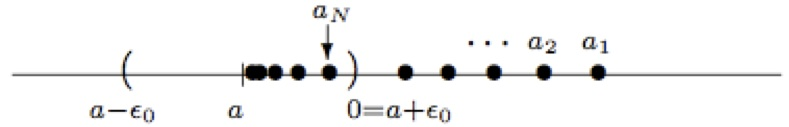
\includegraphics{OrderLimitTH.jpg}
  \caption{If $a_{n} \geq 0$ for all $n \in \mathbb{N}$, then $a\geq0$.}
  %\label{fig:textfig1}
\end{marginfigure}
	\item  The Algebraic Limit Theorem ensures that the sequence $(b_{n} - a_{n})$  converges to $b-a$.  Because $b_{n} - a_{n} \geq 0$, we can apply the results from part (i) to get that $b-a \leq 0$.
	\item  Take $a_{n} = c$ (or $b_{n} = c$) for all $n \in \mathbb{N}$ and apply our results from part (ii).

\end{enumerate}
\end{proof}


Loosely speaking, limits and their properties do not depend at all on what happens at the beginning of the sequence but are strictly determined by what happens as $n$ gets larger.  Changing the values of the first ten (or ten thousand) terms of the sequence has no effect on its eventual limit.


\medskip


\subsection{Exercises}
\noindent
\emph{Exercise 2.3.1.} Show that the constant sequence $(a,a,a,a,...)$ converges to $a$.
\begin{proof}
Since the sequences is constantly $a$, we know that for all $n$:
	$$ |a_n - a| = |a-a| = 0 < \varepsilon $$
	Therefore we can choose $N$ completely arbitrarily since any choice will ensure that $|a_n -a| = 0 < \varepsilon$
\end{proof}

\smallskip

\noindent
\emph{Exercise 2.3.2.}
Let $x_n \geq 0$ for all $n \in N$. 
\begin{enumerate}[(a)]
\item If $(x_n) \to 0$, show that $(\sqrt{x_n}) \to 0$. 
\item If $(x_n) \to x$, show that $(\sqrt{x_n}) \to \sqrt{x}$.
\end{enumerate}

\begin{proof}
\begin{enumerate}[(a)]
\item Let $\varepsilon> 0$.  (We want to show that $|x_n| < \varepsilon$ implies that $|\sqrt{x_n}| < \varepsilon $).

Because $(x_n) \to 0$, we have that there exists $N$ such that $|x_n|= x_n < \varepsilon^2$.  Then we have that for the same $N$, $|\sqrt{x_n}| = \sqrt{x_n} < \sqrt{\varepsilon^2} = \varepsilon$.

As a result, for all $\varepsilon> 0$, there exists $N$ such that $n \geq N$ implies that $|\sqrt{x_n}- 0| < \varepsilon$ and $(\sqrt{x_n}) \to 0$.



\item If $(x_n) \to x$, show that $(\sqrt{x_n}) \to \sqrt{x}$.

Let $\varepsilon > 0$.  We wish to prove that $\exists N$ such that $n \geq N$ implies that $|\sqrt{x_n} - \sqrt{x}| < \varepsilon$.  

$\begin{array} {lcl} 
|\sqrt{x_n} -  \sqrt{x}|& = &|\sqrt{x_n} -  \sqrt{x}| \frac{\sqrt{x_n} +  \sqrt{x}}{\sqrt{x_n} +  \sqrt{x}}\\ 
	& = & \frac{|x_n +  x|}{\sqrt{x_n} +  \sqrt{x}}\\
&\leq	& \frac{|x_n +  x|}{\sqrt{x}}
    \end{array}$
    
    Because $(x_n ) \to x$ and $x>0$, we can choose $N$ such that $|x_n -x | <\varepsilon \sqrt{x}$ whenever $n \geq N$.  This implies that $\forall n \geq N$,
    \[		|\sqrt{x_n} - \sqrt{x}| \leq \frac{|x_n +  x|}{\sqrt{x}} < \frac{\varepsilon \sqrt{x}}{\sqrt{x}} = \varepsilon	\]

\end{enumerate} \end{proof}

\smallskip

\noindent
\emph{Exercise 2.3.3.} (Squeeze Theorem). Show that if $x_n \leq y_n \leq z_n$ for all $n \in N$, and if $\lim x_n = \lim z_n = l$, then $\lim y_n = l$ as well.
\begin{proof}
Since $(x_n) \to l$ $\quad \exists N_{1}$ such that $n \geq N_{1} \implies x_n \in (l- \varepsilon, l + \varepsilon)$.

Since $(z_n) \to l$ $\quad \exists  N_{2}$ such that $n \geq N_{2} \implies z_n \in (l- \varepsilon, l + \varepsilon)$.

Since $x_n \leq y_n \leq z_n$ for all $n \in N$, for $N = \max \{N_1, N_2\}$ then it follows that $y_n \in (l-\varepsilon, l + \varepsilon)$ for all $n \in N$.

\end{proof}

\smallskip


\noindent
\emph{Exercise 2.3.4.}  Show that limits, if they exist, must be unique. In other words, assume $\lim a_n = l_1$ and $\lim a_n = l_2$, and prove that $l_1 = l_2$.
\begin{proof}
\begin{enumerate}[(i)]
	\item    Using the definition of convergence
	\noindent \marginnote{ \begin{proof} $\Rightarrow$ trivial.
		
		$\Leftarrow$ Assume $l_1 \neq l_2 $, then $|l_1 - l_2 |=\varepsilon_{0}$ for some $\varepsilon_{0}> 0$.  However, choosing $\varepsilon < \varepsilon_{0}$, we no longer have $\forall \varepsilon_{0}> \varepsilon > 0$ that $|l_1 - l_2 |< \varepsilon$ since $\varepsilon < |l_1 - l_2 |= \varepsilon_{0}$.  Contradiction.
		\end{proof}}\begin{lemma}  Two numbers $l_1 = l_2 $ are equal iff $|l_1 - l_2 |< \varepsilon$ for all $\varepsilon > 0$.
		\end{lemma} 
	
	Let $\varepsilon > 0$.  Since $(a_n) \to l_1$ and the $(a_n) \to l_2$, there exists $N_1, N_2$ such that $n \geq N_1$ and $n \geq N_2$ implies that $|a_n - l_1| < \varepsilon/2$ and $|a_n - l_2| < \varepsilon/2$  respectively.
	
	Therefore choosing $N = \max\{N_1, N_2\}, \quad n \geq N$ implies:


$\begin{array} {lcl} 
|l_1 - l_2|& = &|l_1 + a_n - a_n - l_2 | \\ 
	& \leq & |l_1 - a_n | +  |a_n - l_2 |\\
	& = & |a_n - l_1 | + |a_n - l_2 |\\
	& < & \frac{\varepsilon}{2} + \frac{\varepsilon}{2} \\
	&=& \varepsilon
    \end{array}$	 
    
    therefore, $l_1 = l_2$.

	\item  By the Algebraic Limit Theorem
	
	$\begin{array} {lclcl} 
\lim (a_n - a_n)& = &\lim (a_n) -\lim (a_n)  &=& l_{1} - l_{2}\\ 
			& = &\lim 0 			&=& 0 \\
    \end{array}	$
    
    Therefore $l_1 - l_2 = 0$ implying that $l_1 = l_2$.
	
\end{enumerate}
\end{proof}

\smallskip


\noindent
\emph{Exercise 2.3.6.} 
\begin{enumerate}[(a)]
\item Show that if $(b_n) \to b$, then the sequence of absolute values $|b_n| $converges to $|b|$.


\item Is the converse of part (a) true? If we know that $|b_n| \to |b|$, can we deduce that $(b_n) \to b$?
\end{enumerate}

\begin{proof}
\begin{enumerate}[(a)]
\item We wish to show that $\forall \varepsilon > 0 \quad |b_n - b| < \varepsilon  \implies ||b_n| - |b|| < \varepsilon$.

$\begin{array} {rcrcl} 
|b_n|& = &|b_n - b + b|  &\leq & |b_n - b| + |b|\\ 
	&&	|b_n| - |b|	& \leq & |b_n - b|	\\
||b_n| - |b|| &\leq&    ||b_n - b|| &=& |b_n - b|\\
    \end{array}	$
    
    Since $(b_n) \to b  \quad \exists N$ s.t. $n \leq N \Rightarrow |b_n - b| < \varepsilon$.
    
    Therefore, for the same $N$, $n \leq N$,
    $$ ||b_n| - |b|| \leq     |b_n - b| < \varepsilon $$
    and $|b_n| $converges to $|b|$.
    
\item No, the converse is not true.
\end{enumerate}
\end{proof}

\smallskip


\noindent
\emph{Exercise 2.3.7.} 
\begin{enumerate}[(a)]
	\item Let $(a_n)$ be a bounded (not necessarily convergent) sequence, and assume $\lim b_n = 0$. Show that $\lim(a_n b_n ) = 0$. Why are we not allowed to use the Algebraic Limit Theorem to prove this?

\item Can we conclude anything about the convergence of $(a_n b_n)$ if we assume that $(b_n)$ converges to some nonzero limit $b$?
%\item Use $(a)$ to prove Theorem 2.3.3, part (iii), for the case when $ a = 0$.
\end{enumerate}

\begin{proof}

\begin{enumerate}[(a)]
	\item   Because $(a_n)$ is bounded, there exists $M > 0$ such that $|a_n| \leq M \quad \forall n \in N$.
	
	Furthermore since $(b_n) \to 0$, there exists $N$ such that $n \geq N$ implies that $|b_n| \leq \frac{\varepsilon}{M}$.
	
	Then the sequence $(a_n b_n) $ is such that for $n \geq N$
	$$ |a_n b_n | \leq |a_n| |b_n| < M \frac{\varepsilon}{M} = \varepsilon $$
	
	
	and $a_n b_n  \to 0$
	
	
	We cannot use the Algebraic Limit Theorem to prove this since not both sequences are convergent.
	
	
	

\item No we cannot conclude anything about the sequence. 
\end{enumerate}
\end{proof}

\noindent
\emph{Exercise 2.3.10.}
If $(a_n) \to 0$ and $|b_n - b| \leq a_n$ then $(b_n) \to b$

\begin{proof}
	We must have $a_n$ positive since there always exists a positive value less than $a_n$.  Therefore $|a_n| = a_n$.
	
	If $(a_n) \to 0$ then $\forall \varepsilon > 0 \quad \exists N \quad \text{such that} |a_n | = a_n < \varepsilon$.
	
	Then the the above inequality $|b_n - b| \leq a_n < \varepsilon$ when $n \geq N$.   Therefore $(b_n) \to b$.
\end{proof}


\noindent
\emph{Exercise 14.}

  If $\{s_{n}\}$ is a complex sequence, define its arithmetic means $\sigma_{n}$ by
 $$  \sigma_{n} = \frac{s_{0} + s_{1} + \cdots + s_{n}}{n+1} \qquad (n=0,1,2,\ldots) $$
 
 \begin{enumerate}[(a)]
 	\item  If $\lim s_{n} = s$, prove that $\lim \sigma_{n} = s$.
	
	\begin{proof}
			Let $\varepsilon >0$.
			
			If $\lim s_{n} = s$  then the sequence is bounded, that is, there exists an $M >0$ such that $$ |s_n - s| < M $$
			
			Furthermore, there exists an $N_{1} \in \mathbb{N}$ such that $n \geq N_{1}$ implies that $$  |s_n - s|< \frac{\varepsilon}{2} $$
			
			Therefore for $n \geq N_{1}$ we have that 
			
			\begin{eqnarray*}
|\sigma_n - s|  &=& \big|\frac{s_0 + s_1 + s_2 + \cdots + s_n}{n+1}  - s\big|  \\
   	&=& \big|\frac{s_0 + s_1 + s_2 + \cdots + s_n - (n+1)s}{n+1}\big| \\
   &=& \big|\frac{(s_0-s) + (s_1 -s) + (s_2 -s)  + \cdots + (s_n - s)}{n+1}\big| \\
   &\leq & \big|\frac{(s_0-s) + (s_1 -s) +\cdots + (s_{N_{1} - 1} -s) }{n+1}\big|  + \big|\frac{(s_{N_{1}} -s) + \cdots + (s_n - s)}{n+1}\big| \\
   &<& \frac{(N_{1} - 1 )(M)}{n+1}  + \frac{\varepsilon}{2}\frac{(n - N_{1})}{n+1}\\
   &<& \frac{(N_{1} - 1 )(M)}{n+1}  + \frac{\varepsilon}{2}
\end{eqnarray*}

Note that in the last line we used the fact that for $n \geq N_1$, $\frac{(n - N_{1})}{n+1} < 1$. 


But $N_{1}$ and $M$ are fixed meaning they are simply constants.  Since the sequence $\{\frac{1}{n+1}\} \rightarrow 0$ we can fix the quantity $\frac{(N_{1} - 1 )(M)}{n+1}$ to be arbitrarily small.

Choose $N_2$ such that $n \geq N_2$ implies that $$ \frac{(N_{1} - 1 )(M)}{n+1} < \frac{\varepsilon}{2} $$




Finally, let $N = \max\{N_1, N_2\}$.   Then $n \geq N$ implies that 


\begin{eqnarray*}
|\sigma_n - s|  &<& \frac{(N_{1} - 1 )(M)}{n+1}  + \frac{\varepsilon}{2}\\
		&<& \frac{\varepsilon}{2} + \frac{\varepsilon}{2} \\
		&=&  \varepsilon
\end{eqnarray*}

as desired.	
	\end{proof}
	\item  Construct a sequence $\{s_{n}\}$ which does not converge although $\lim \sigma_{n} = 0$.
	
	\noindent
	\emph{Solution:}   The sequence $\{s_{n}\} = (a, -a, a, -a, a, -a, a, -a, a, \ldots )$ does not converge but the sequence $\{\sigma_{n}\}$ converges to $0$.
 \end{enumerate}

 


\smallskip

\section{The Monotone Convergence Theorem }
We showed previously that convergent sequences are bounded.  While the converse is not necessarily true, if a sequence is bounded as well as monotonic, then it converges.


\begin{definition}Increasing sequence:  A sequence $\{a_{n}\}$ is \emph{increasing} if $a_{n} \leq a_{n+1}$ for all $n \in \mathbb{N}$ and \emph{decreasing} if $a_{n} \geq a_{n+1}$ for all $n \in \mathbb{N}$.  A sequence is $monotone$ if it is either increasing or decreasing. \end{definition}

\begin{theorem}  [The Monotone Convergence Theorem] If a sequence is monotone and bounded, then it converges.
\end{theorem}

\begin{proof}
	Let $(a_n)$ be monotone and bounded.
	WLOG assume $(a_n)$  is increasing and consider the set of points $\{a_n : n \in \mathbb{N}\}$.
	
	By assumption, the set is bounded.  By the axiom of completeness, the set has a supremum.  Let $s = \sup\{a_n : n \in \mathbb{N}\}$.
	
	We claim that $\lim (a_n) = s$.
	
	Let $\varepsilon > 0$.  Because $s$ is the least upper bound of $\{a_n : n \in \mathbb{N}\}$, $s- \varepsilon$ is not an upper bound, so there exists  a point in the sequence call it $a_N$ such that $s-\varepsilon < a_N$.
	
	Now the fact that $(a_n)$ is increasing implies that if $n \geq N$ then $a_N \leq a_n$.
	
	Hence,
	$$ s- \varepsilon < a_N \leq a_n < s < s+\varepsilon $$
	which implies that $|a_n  - s| < \varepsilon$ for all $n \in \mathbb{N}$.
\end{proof}

Note that the Monotone Convergence Theorem is extremely useful since it asserts the convergence of a sequence without explicit mention of the actual limit.

Also note that the Monotone Convergence Theorem follows from the Axiom of Completeness.

\subsection{Exercises}

	\emph{Exercise 2.4.2.}
		\begin{enumerate}[(a)]
			\item Prove that the sequence defined by $x_1 = 3$ and 
				\[		x_{n+1} = \frac{1}{4-x_n}\]
				converges.
			\item Now that we know $\lim x_n$ exists, explain why $\lim x_{n+1}$ must also exist and equal the same value.
			\item Take the limit of each side of the recursive equation in part (a) of this exercise to explicitly compute  $\lim x_n$.
		\end{enumerate}
		
		\begin{proof}
			\begin{enumerate}[(a)]
				\item  
				\begin{enumerate}[(i)]
					\item The first few terms of the sequence are $x_n = 3, 1, \frac{1}{3}, \frac{3}{11}, \ldots$.  Then we can guess that the sequence is decreasing ($x_{n+1}< x_{n} \quad \forall n$)  and we can prove it by induction.
				
				For $n=1$,  $x_{2}< x_{1}$ since $1 <3$.
				
				For $n=k$, assume that $x_{k+1} < x_{k}$.
				
				Then when $n=k+1$, we want to be able to show that $x_{k+2} =\frac{1}{4-x_{k+1}} < x_{k+1} = \frac{1}{4-x_{k}}  $.   Using the inductive hypothesis, we have that
				
				
				\begin{eqnarray*}
x_{k+1}  &< & x_{k} \\
   	-x_{k+1}  &>& -x_{k} \\
 4-x_{k+1}  &>&4 -x_{k}\\
    \frac{1}{4-x_{k+1}}  &<&\frac{1}{4 -x_{k}}\\
   x_{k+2}  &< & x_{k+1} \\
\end{eqnarray*}

as desired.
				\item We can see that $(x_n)$ is bounded above by $3$ but we would like to prove that it is bounded below by $0$.  Again we can prove this by induction, showing that $x_n > 0 \quad \forall n$.
				
				Clearly for $n=1$, $x_1 = 3 >0$.
				Then assume for $n=k$, that $x_k >0$.
				
				To show this for $n = k+1$, note that we have that $3>x_k>0$.  This implies that $x_{k+1} = \frac{1}{4-x_k}$  is positive.  Therefore $x_{k+1}>0$ as desired.
				
				
				Since $(x_n)$ is decreasing and bounded below by $0$, we have by the MTC that the sequence is convergent.
				
								\end{enumerate}
				
				\item Since $ (x_n)$ is bounded and decreasing, $(x_{n+1})$ must also be bounded and decreasing, then by the MTC it must also be convergent.
				
				Furthermore since $(x_n) \to L$, it must be that $\forall \varepsilon >0 \quad \exists n \in N \quad st \quad n \geq N$ implies that $|x_n - L| <\varepsilon$.  However, notice that for $(x_{n+1})$ this same $N$ works since $n+1> n \geq N$ and therefore $|x_{n+1} - L| <\varepsilon$ and both sequences converge to the same limit.
				
							\item By part (b), we have that  $\lim x_n = \lim x_{n+1} = L$. Furthermore, by the Algebraic Limit Theorem we can deduce that $L = \lim x_{n+1} = \lim \frac{1}{4-x_n} = \frac{1}{4-L}$ and we have that $L$ satisfies the equation $L^2 - 4L +1 =0$.  Solving for $L$ we have that $L = 2 \pm \sqrt{3}$, however since $3$ is an upper bound for the sequence, we must have that $L= 2 - \sqrt{3}$.
			\end{enumerate}
		
		\end{proof}
		
\noindent		
\emph{Exercise 2.4.3.}Using the same methods prove that the following sequence is convergent and find its limit.
	$$y_{n+1} = 4 - \frac{1}{y_n}	\qquad y_1 = 1$$
	
	\begin{proof}
		\begin{enumerate}[(i)]
			\item Monotone.  Looking at the first few terms of the sequence again, we can see that it is increasing that $y_n \leq y_{n+1} \quad \forall n$.  To prove this we use induction.
				
				For $n=1$, $y_1 \leq y_2$ since $1 < 3$.
				
				Assume that for $n=k$, it is true that $x_{k} \leq x_{k+1}$.
				
				Then for $n = k+1$, 
				\begin{eqnarray*}
x_{k}  &\leq & x_{k+1} \\
   	-x_{k}  &\geq& -x_{k+1} \\
    \frac{1}{-x_{k}}  &\leq&\frac{1}{ -x_{k+1}}\\
      4- \frac{1}{-x_{k}}  &\leq&4- \frac{1}{ -x_{k+1}}\\
   x_{k+1}  &\leq& x_{k+2} \\
\end{eqnarray*}

as desired.

\item Bounded.  It is clear that the sequence is bounded below by $1$ however, now we wish to prove that it is bounded above by $4$.  For $n=1$ this is trivial.  Assume then that $1< x_k < 4$.  Then $x_{k+1}<4$ as well, since we can see that $0 \geq \frac{1}{x_k}\leq 1$.

\item Limit.  Note that $\lim y_n = \lim y_{n+1} = y$.  Then $y = \lim y_{n+1} =  \lim (4 - \frac{1}{y_n}) = 4 - \frac{1}{y}$.  By this relation we have that $y^2 - 4y + 1 =0$ with roots $y = 2 \pm \sqrt{3}$.  However, since the sequence is bounded below by 1, we have that $y = 2 + \sqrt{3}$.

				
		\end{enumerate}
	\end{proof}
	
\emph{Exercise 2.4.4.}  Prove that the sequence $x_n = \sqrt{2}, \sqrt{2\sqrt{2}}, \sqrt{2\sqrt{2\sqrt{2}}}, \ldots$
	converges and find the limit.
	
	\begin{proof}
	First, define the sequence recursively:
	$$  x_{n+1} = \sqrt{2 x_n} \qquad x_n = \sqrt{2} $$
		\begin{enumerate}[(i)]
		
			\item Monotone Increasing  ($x_{n} < x_{n+1}\quad \forall n$).  For $n=1, \quad \sqrt{2} < \sqrt{2\sqrt{2}}$. Then assume that for $n=k$, $x_k < x_{k+1}$.
			
			Using the Inductive hypothesis
			\begin{eqnarray*}
x_{k}  & <& x_{k+1} \\
   	2x_{k}  &<& 2x_{k+1} \\
    \sqrt{2x_{k}}  &<&\sqrt{ 2 x_{k+1}}\\
    x_{k+1}  & <& x_{k+2}
\end{eqnarray*} as desired.

\item Bounded.  We wish to prove that the sequence is bounded above by 2.
For $x_1$ this is trivial.  Assume that $x_k < 2$.
Then 
\marginnote{Notice that here we take the limit under a square root which is not covered in the Algebraic Limit Theorem.  We therefore use Exercise 2.3.2 to support our argument.}
\begin{eqnarray*}
x_{k}  & <& 2 \\
   	2x_{k}  &<& 4 \\
    \sqrt{2x_{k}}  &<&\sqrt{ 4}\\
 & <& 2 \\
 x_{k+1}  & <& 2
\end{eqnarray*} as desired.   


\item Limit.  Note that $x = \lim x_n = \lim x_{n+1}$.  Therefore we have that $x = \lim x_{n+1} = \sqrt{2x}$ and we have that $x^2 - 2x = 0$.  Therefore $x = 2$
		\end{enumerate}
	\end{proof}
	
	\emph{Exercise 2.4.6.} Let $(a_n)$ be a bounded sequence.
	
	\begin{enumerate}[(i)]
	\item We define the sequence $y_n = \sup \{a_k : k \geq n\}$.  Prove that $\lim y_n$ exists
	\item Define the sequence $z_n = \inf \{a_k : k \geq n\}$ and prove that it converges
	\item Show that $\lim \sup a_n = \lim \inf a_n$ iff $\lim a_n$ exists and that all sequences converge to the same limit.
	\end{enumerate} % COMPLETE


\section{Subsequences and Bolzano-Weierstrass Theorem}

\begin{definition}Subsequences:  Given a sequence $\{p_n\}$ consider a sequence $\{n_k\}$ of positive integers such that $n_1 < n_2 < n_3 < \cdots$.  Then the sequence $\{p_{n_i}\}$ is called a \emph{subsequence} of $\{p_n\}$.  If $\{p_{n_i}\}$ converges, its limit is called a \emph{subsequential limit} of $\{p_{n}\}$.
\end{definition}
\medskip
Note:  It is clear that $\{p_{n}\}$ converges to $p$ if and only if every subsequence of $\{p_{n}\}$ converges to $p$. 

Notice also that the order of the terms in the subsequence is the same as in the original sequence and that repetitions are not allowed.

\begin{theorem} Subsequences of a convergent sequence converge to the same limit as the original sequence.\end{theorem}

\begin{proof} 
Assume the sequence $(x_n) \to L$ and let $(x_{n_j})$ be a subsequence of this sequence.  
Let $\varepsilon > 0$.  Then there exists an $N$ such that $n \geq N$ implies that $|x_n - L| < \varepsilon$.  But since $n_j \geq j$ this same $N$ works for the subsequence as well.  To be more precise, $j\geq N$ implies that $n_j \geq N$ and that $|x_{n_j} - L| < \varepsilon$ as desired.


\end{proof}

This theorem can sometimes provide a very useful proof for divergence of a sequence.  If we can find two subsequences that converge to two different limits, then we can rigorously conclude that the original sequence diverges.

Furthermore, this theorem can be applied to infinite series to show that infinite sums are associative which we will see later.

\begin{example} Let $0 < b< 1$.  Because $b >b^2 > b^3 > b^4 > \ldots > 0$ the sequence is decreasing and bounded below.  By the MTC the sequence converges to some limit $l$ satisfying $b > l \geq 0$.   Notice however that $(b^{2n})$ is a subsequence, so by the above theorem $(b^{2n}) \to l$. But $(b^{2n}) = (b^n)( b^n)$ so by the Algebraic limit theorem, $(b^{2n}) \to l \cdot l = l^2$.  Because limits are unique $l^2 = l$ and therefore $l=0$.
\end{example}

\begin{example}
Consider the sequence 
$$\big( 1, - \frac{1}{2}, \frac{1}{3}, -\frac{1}{4}, \frac{1}{5}, -\frac{1}{5}, \frac{1}{5}, -\frac{1}{5}, \frac{1}{5}, -\frac{1}{5},\ldots	\big)$$

We can show that the sequence is divergent since we can provide two subsequences, namely:
$$ \big( \frac{1}{5}, \frac{1}{5}, \frac{1}{5}, \frac{1}{5},  \ldots \big) \quad \text{and} \quad \big( -\frac{1}{5},-\frac{1}{5},-\frac{1}{5},-\frac{1}{5}, \ldots \big) $$

that converges to two different limits.
\end{example}

\begin{theorem}\newthought{Bolzano-Weierstrass Theorem:} Every bounded sequence contains a convergent subsequence.\end{theorem}

\begin{proof}
Let $(a_n)$ be a bounded sequence such that $|a_n| \leq M$ for all $n$.  If we were to bisect the closed interval $[-M, M]$ into $[-M, 0]$ and $[0,M]$ where the midpoint will be in both intervals.  Now it must be that at least one of these closed intervals contains infinitely many terms of the sequence $(a_n)$.  Select the half for which this is the case and labeling it $I_1$.  Then let $a_{n_1}$ be some point in the sequence satisfying $a_{n_1} \in I_1$.

Now bisect $I_1$ and again select the half with infinitely many $(a_n)$ and call it $I_2$.  Then again select a point $a_{n_2} \in I_2$ such that $n_2> n_1$.

Continuing in this way by constructing $I_{k}$ by halving $I_{k-1}$ and choosing the half with infinitely many terms of the sequence $(a_n)$ and then selecting $a_{n_k} \in I_{k}$ such that
\[	n_k  > n_{k-1} > n_{k-2} > \cdots > n_{2} > n_{1}	\]


We want to show that $(a_{n_j})$ converges but we first need to find a candidate for the limit.

Note that 
\[	I_1 \supseteq I_2 \supseteq I_3 \supseteq I_4 \supseteq	\cdots \]
and that each $I_i$ is closed.

By the NIP, $\exists x \in \mathbb{R}$ such that $x \in I_k \forall k$ and therefore that $x \in \cap I_i $.


Let $\varepsilon >0$.  By construction, the length of $I_k = M (\frac{1}{2})^{k-1}$  which $\to 0$ as $k \to \infty$.

Therefore $\exists N$ s.t.  $k \geq N \implies |I_k| = M (\frac{1}{2})^{k-1} < \varepsilon$.  However $x \in I_k$ and $a_{n_k} \in I_k$ which is becoming arbitrarily small.  As a result, $|x-a_{n_k}|< \varepsilon$.

\end{proof}

\section{The Cauchy Criterion}  
\newthought{Cauchy Sequence:}  A sequence $(a_n)$ is called a \emph{Cauchy sequence} if, for every $\varepsilon >0$ there exists an $N \in \mathbb{N}$ such that whenever $m,n \geq N$ it follows that $|a_n - a_m| < \varepsilon$

That is, a sequence is Cauchy if, for every $\varepsilon$, there is a point in the sequence after which all the terms are closer to each other than the given $\varepsilon$.  To spoil the surprise, we will argue that Cauchy sequences are convergent and that convergent sequences are Cauchy.  This, like the Monotone Convergence Theorem, allows us to prove that a sequence converges without having explicit knowledge of what the limit might be. 


\begin{lemma} Cauchy Sequences are bounded.\end{lemma}

\begin{proof}
	Given $\varepsilon = 1$, there exists an $N$ such that $|x_m - x_n| <1$ for all $m,n \geq N$.  
	As a result \marginnote{Note that $|x_n| = |x_n + x_N - x_N| \leq |x_n -x_N| + |x_N| < \varepsilon + |x_N|$}  $|x_n| < |x_N| + 1$ for all $n \geq N$. Note that there were finitely many terms before $x_N$ in the sequence. Therefore let
	
	
	\[	M	= max \{|x_1|,|x_2|, |x_3|, |x_4|, \cdots, |x_N| + 1 \}\]
	And this value is a bound for the sequence.
\end{proof}


\begin{theorem}\newthought{Cauchy Criterion:} A sequence converges iff it is a Cauchy sequence. \end{theorem}

\begin{proof}
	$\Longrightarrow$.  This we can prove by applying the triangle inequality. Assume that a sequence $(x_n)$ converges to a limit $x$.   Then $\forall \varepsilon >0$, there exists an $N$ such that $n,m \geq N$ implies that 
	\[ |x_n -x | < \varepsilon/2	\qquad 	|x_m - x| < \varepsilon/2	\]
Applying the triangle inequality, we can state that 

$$
\begin{array}{rcl}
|x_n - x_m| &=& |x_n - x  + x - x_m| ,\\
&\leq & |x_n - x| + |x - x_m|,\\
& < & \varepsilon\\
\end{array}
$$

as desired.   

	$\Longleftarrow$.  So the other direction is a lot harder to prove and we have to invoke Bolzano-Weierstrass to get our result.
	
	Assume we have a Cauchy sequence $(x_n)$.  By the lemma above we know that is it bounded and so by BW we know that it contains a convergent subsequence.   Let us call this subsequence $x_{n_k}$ and call its limit $x$.  
	
	The idea here is that because the sequence is Cauchy, we know that elements in the "tail" end of the sequence are getting closer together.  But because the terms in the subsequence are getting closer to the limit $x$, we can force each value to be less that $\varepsilon/2$ and apply the triangle inequality.
	
	So let $\varepsilon >0$.
	
		Because $(x_n)$ is Cauchy there is an $N$ such that $m,n \geq N$ implies that \[|x_n - x_m|<\varepsilon/2\].  We also have that the subsequence converges so we can choose an index, let say $n_K$, such that $n_K \geq N$ implies that 
		\[	|x_{n_K} - x|<\varepsilon/2 \]
		
		
		We also have to be sure that the index $n$ we choose is greater than $n_K$ so that 
		
				$$
				\begin{array}{rcl}
|x_n - x| &=& |x_n - x_{n_K}  + x_{n_K} - x| ,\\
&\leq & |x_n - x_{n_K}| + |x_{n_K} - x_m|,\\
& < & \varepsilon
\end{array}
$$
	
\end{proof}



One important thing to note is that many of our significant results up to this point rely heavily on the Axiom of Completeness.

The AoC was what allowed us to prove the NIP which allowed us to prove Bolzano-Weierstrass which allowed us to prove the Cauchy Criterion.  Furthermore the AoC also gave us the Monotone Convergence Theorem.

$$
\begin{array}{rcl}
AoC &\implies & NIP \implies BW \implies CC ,\\
&\implies & MCT,\\
\end{array}
$$

Also note that we could have begun this chain with ANY of these axioms and arrived at the others as a result.  This is pretty remarkable.  In other words all of these statements are equivalent and that assuming any one of them to be true, means that we can derive the others.   This is because all of these statements essentially say the same thing : that the field of real numbers is $complete$.   Remember how we could not show the AoC in the field of rational numbers.  This is because the rationals did not contain a certain property, independent of the field and order axioms, that forced this result to be true.  In the next section we try to define more explicitly what this "completeness" property is and how it relates to the topology of the field in question.


\section{Infinite Series}


\newthought{Infinite Series:}  Let $(b_n)$ be a sequence.  An infinite series is an expression of the form
		\[\sum_{n=1}^{\infty} b_n = b_1 + b_2 + b_3 + \cdots \]
		
		The sequence of \emph{Partial sums} of the series $(s_m)$ is defined as 
			\[s_m = b_1 + b_2 + b_3 + \cdots + b_m \]
			
		We say that the series $\sum_{n=1}^{\infty} b_n$ \textsc{converges} if its sequence of partial sums converges to some limit B and we denote this limit as $\sum_{n=1}^{\infty} b_n  = B$.
		Specifically,
		\[\sum_{n=1}^{\infty} b_n = B \qquad \text{means that} \qquad \lim s_n = B\]
		
		
		\begin{dangerousbend}
			It is important to keep a distinction between 
				\begin{itemize}
					\item The sequence of \emph{terms}: $(b_1, b_2, b_3, \ldots)$ and
					\item The sequence of \emph{partial sums}:  $(s_1, s_2, s_3, \ldots)$ where $s_n = b_1 +  \cdots + b_n$
				\end{itemize}
		\end{dangerousbend}
		
		Nonetheless it is this close relationship between series and sequences that allows us to apply much of our previous knowledge to them.
		
		
		\begin{theorem}\newthought{Theorem: Algebraic Limit Theorem for Series}
		If $\sum_{n=1}^{\infty} a_n = A$ and $\sum_{n=1}^{\infty} b_n = B$ then,
			\begin{enumerate}[(1)]
				\item $\sum_{n=1}^{\infty} c a_n = cA$
				\item $\sum_{n=1}^{\infty} a_n + b_n = A + B$
			\end{enumerate}
		\end{theorem}
		
		\begin{proof}
		\end{proof}
		
		\begin{theorem} \newthought{Cauchy Criterion for Series}
		The series $\sum_{n=1}^{\infty} a_n$ converges 
		
		$$iff$$
		
		
		 $\forall \varepsilon > 0$ there exists an $N \in \mathbb{N}$ such that $n>m\geq N$ implies that $|a_{m+1} + a_{m+2} + \cdots + a_n| < \varepsilon$
		\end{theorem}
		
		
	\begin{proof}  \end{proof}
	
	This can help us prove some basic facts about series.
	
	
	\begin{theorem} If the series $\sum_{n=1}^{\infty} a_n$ converges then $(a_k) \to 0$.  \marginnote{The converse statement is NOT true!! Take for example the harmonic series.}
	\end{theorem}
	
	\begin{proof}  \end{proof}
	
	\begin{theorem}\newthought{The Comparison Test}  Assume that $(a_n)$ and $(b_n)$ are sequences where $0 \leq a_n \leq b_n$  for all $\mathbb{N}$
		\begin{enumerate}
			\item If $\sum_{n=1}^{\infty} b_n$ converges, then $\sum_{n=1}^{\infty} a_n$ converges.
			\item If $\sum_{n=1}^{\infty} a_n$ diverges, then $\sum_{n=1}^{\infty} b_n$ diverges.
		\end{enumerate}
	\end{theorem}
	
	
	
	\begin{proof}  \end{proof}
	
	Remember also that statements about the convergence of a sequence (or series) only care about the tail ends of the sequence.  In other words, we can change around a few things about some finite number of initial terms without affecting the infinite behavior of the sequence (or series).
	
	Because the Comparison Test is about deducing the behavior of a series in comparison to another, it might be a good idea to have an arsenal of basic series to which we can compare another. 
	
	\newthought{Absolute Convergence:}  If $\sum_{n=1}^{\infty} |a_n|$ converges then we say that $\sum_{n=1}^{\infty} a_n$ converges absolutely.  On the other hand if $\sum_{n=1}^{\infty} a_n$ converges and $\sum_{n=1}^{\infty} |a_n|$ diverges we say that the series \emph{converges conditionally}.
	
	
	\begin{theorem}\newthought{Absolute Convergence Test}
	If the series $\sum_{n=1}^{\infty} |a_n|$ converges, then $\sum_{n=1}^{\infty} a_n$ converges as well.
	\end{theorem}  \marginnote{The converse of this theorem is also false!}
	\begin{proof}  \end{proof}
	
	
	\begin{theorem}\newthought{Alternating Series Test}  Let $(a_n)$ be a sequence satisfying,
	
	\begin{enumerate}
		\item The sequence is monotone decreasing:  $a_1 \geq a_2 \geq a_3 \geq \cdots a_n \geq a_{n+1} \geq \cdots $ and
		\item $(a_n) \to 0$
	\end{enumerate}
	
	
	Then the alternating series $\sum_{n=1}^{\infty} (-1)^{n+1} a_n$ converges.
	\end{theorem}
	\begin{proof}  \end{proof}
	
	\begin{theorem}\newthought{Ratio Test}
	Given a series $\sum_{n=1}^{\infty} |a_n|$, with $a_n \neq 0$, the ratio test states that if $(a_n)$ satisfies 
	\[		\lim \big|\frac{a_{n+1}}{a_n}	\big| = r < 1\]
	then the series converges absolutely (and therefore converges).
	\end{theorem} 
	\begin{proof}  \end{proof}
	
	
	\subsection{Rearrangements}
		Imagine that we were to permute the terms in a sum into some other order such that all of the original terms eventually appeared in the new order and such that no terms were repeated.  Clearly there are an infinite number of possible rearrangements of a series.  
		
		More formally,
		
		\newthought{Rearrangement}  Let  $\sum_{n=1}^{\infty} a_n$ be a series.  Another series  $\sum_{n=1}^{\infty} b_n$ is called a rearrangement of  $\sum_{n=1}^{\infty} a_n$ if there exists a bijection from the indices of the series such that $b_{f(k)} = a_{k}$ for all $k$.
		
		It should be noted however, that rearrangements of series DO NOT always converge to the same limit as the original series.  This is only true for absolutely convergent series as we will now prove.
		
		
		\begin{theorem}
	If $\sum_{n=1}^{\infty} a_n$ converges absolutely, then any rearrangement of the series converges to the same limit.
	\end{theorem} 
	\begin{proof}  \end{proof}
	
	This theorem should make clear that absolute convergence is an extremely desirable property when manipulating series.  However it should be noted that conditional convergence has this amazing and not at all obvious property which we attribute to Riemann.
	
	
	\begin{theorem}\newthought{Riemann}
	If $\sum_{n=1}^{\infty} a_n$ converges conditionally, then we can always find a  rearrangement of the series that converges to ANY real number.
	\end{theorem} 
	\marginnote{Not required to know the proof of this statement although it follows from 3.54 of Rudin}
		
		
\setcounter{chapter}{3}
\chapter{Chapter Three:  Basic Topology}


\setcounter{section}{0}
\setcounter{theorem}{0}
\setcounter{definition}{0}		
		

\section{Metric Spaces}

\textsc{Metric Spaces}  A set X whose elements, we shall call points, is said to be a metric space if with any two points p and q of X there is associated a real number called the distance from p to q such that:

\begin{itemize}
	\item $d(p,q) > 0$ if $p \neq q  ; d(p,p) = 0$
	\item $d(p,q) = d(q,p)$
	\item $d(p,q) \leq d(p,r) + d(r,q)$ for any $r \in X$  (Triangle Inequality)
\end{itemize}

\newthought{Examples of Metric Spaces:}
\begin{enumerate}
	\item Let $X$ be any set and define
		
\begin{displaymath}
   d(p,q) = \left\{
     \begin{array}{lr}
       0 & : if q \neq q \\
       1 & : if p =q
     \end{array}
   \right.
 \end{displaymath} 
 
 \item Q or E with $d(p,q) =|p-q|$ is a metric space
 
 \item  $\mathbb{R}^2 = \{x_1 x_2 \in \mathbb{R}\}$ with
 \[d(\vec{x}, \vec{y}) = ||\vec{x}- \vec{y}|| = \sqrt{(x_1 - y_1)^2  + (x_2 - y_2)^2} \]  is a metric space.
 
 \item  The most important examples of metric spaces from out standpoint are the euclidean spaces $R^k$ with the distance function defined as above.  The rules of operations on norms  in $R^k$(reviewed below) show that the conditions of a metric space are satisfied.
		
\end{enumerate}

Also note that every subset of a metric space, is itself a metric space under that same distance function.  Thus every subset of euclidean space is a metric space.


\newthought{Definitions:}
\begin{itemize}

	\item A  \textsc{segment (a,b)} is the set of real numbers x such that  $a<x<b$ 
	\item An \textsc{interval  [a,b]} is the set of real numbers x such that  $a\leq x \leq b$	
	
	\item A \textsc{k-cell} is the set of points in $R^k$ such that  $a_i\leq x \leq b_i$ for $1 \leq i \leq k$, given that $a_i < b_i$ for every $1 \leq i \leq k$.
	\item An \textsc{Open (or Closed) Ball} with a center at x and a radius r is the set of all points y such that $|x-y|< r$
	\item A set E is \textsc{convex} if $\lambda y + \lambda(1-z) \in E$ given $y,z \in E$ and $0< \lambda < 1$.
	\item A \textsc{neighborhood} a point p with radius r is the set of all points q such that $d(p,q) < r$
	
	\item A \textsc{Limit Point of E}  is a point p such that every neighborhood of p contains a point q, $q \neq p$ such that $q \in E$
	\item An \textsc{Isolated Point}  is a point $p\in E$ such that p is not a limit point of E (that is, there is a neighborhood of p that contains no other points of E)
	\item A set E is \textsc{Closed} if it contains all of its limit points.
	\item An \textsc{Interior Point}  is a point $p\in E$ such that there exists a neighborhood (N) at p where $N \subset E$
	\item A set E is \textsc{Open} if all of its points are interior points.   \marginnote{The notion of being "open" is relative to the metric space that contains the subset.}
	\item The \textsc{Complement} of a set E is the set of all points $p \in X$	such that $p \notin E$
	\item A set E is \textsc{Bounded} if there exists a real number M and a point $p \in X$ such that $d(p,q) < M$ for all $q\in E$
	\item A set E is \textsc{Dense} in X if for all $p\in X$, p is either a limit point of E or $p \in E$	
	
	\end{itemize}

\newthought{Every Neighborhood is an open set. That is, open balls are open.}

\begin{proof}
Consider a neighborhood $E = N_r (p) $ and let q be any point of E.  Then there is a positive real number h such that 
\[d(p,q) = r-h\]
For all points $s$ such that $d(q,s)<h$, we have then that
\[d(p,s) \leq d(p,q) + d(p,s) < r-h+h = r\]
so that $s\in E$.  Thus $q$ is an interior point of E and therefore E is open. 
\end{proof}

\newthought{Theorem:} If p is a limit point of a set E, then every neighborhood of p contains infinitely many points of E.

\begin{proof}
We proceed with a proof by contradiction.  Suppose that there is a neighborhood N of p which contains only a finite number of points of E.   Let $q_1, q_2, \ldots , q_n$ be those points of $N \cap E$, which are distinct from p, and put
\[r = \min_{1\leq m \leq n} d(p,q_m)\]
The minimum of a finite set of positive numbers is clearly positive so that r>0.\\ 

The neighborhood $N_{r}(p)$ contains no point $q$ of E such that $q \neq p$ so that p is not a limit point of E.  This contradiction established the theorem.
\end{proof}

\newthought{Corollary:} A finite point set has no limit points.

\newthought{Theorem:} A set E is open $\iff$ its complement is closed.

\begin{proof}
($\Leftarrow$)  Assume that $E^c$ is closed and say that $p \in E$.  Then $p \notin E^c$, so $p$ cannot be a limit point of $E^c$.  Hence, there exists an $r>0$ such that $B_r (p)$ does not contain any points of $E^c$.  Then $B_r (p) \subset E$, p is an interior point of E and E is open.\\
($\Rightarrow$)  Assume that E is open.  Let $p$ be a limit point of $E^c$.  Since $p$ is a limit point of  $E^c$ then every neighborhood of $p$ contains a point of  $E^c$ other than p.   But then for every neighborhood of p, $B_r (p) \not \subset E$.  Therefore $p$ is not an interior point of $E$, and since $E$ is open, this implies that $p \in E^c$.
\end{proof}

%\newtheorem{Theorem:}  Let (X,d) be a metric space and let A be any set.   
%\begin{itemize}
	%\item 
%\end{itemize}


\section{Compactness}

Some heuristic remarks are helpful only to a subset of readers. (Maybe that's true of all heuristics, as a meta-heuristic - if everyone accepts a rough explanation, it's something rather more than that.)

Non-compactness is about being able to "move off to infinity" in some way in a space. On the real line you can do that to the left, or right: but bend the line round to fill all but one point on a circle (which is compact) and you see the difference having the "other point" near which you end up. This example of real line versus circle is too simple, really. Another way you can "go off to infinity" in a space is by having paths branching out infinitely.

Compactness is a major topological concept because the various ways you might try to "trap" movement within a space to prevent "escape" to infinity can be summed up in a single idea (for metric spaces, let's say). The definition by open sets is cleaner, but the definition by sequences having to accumulate on themselves (not necessarily to converge, but to have at least one convergent subsequence) is somewhat quicker to say. If you restrict attention to spaces that are manifolds, you can think of continuous paths and whether they have to wind back close to themselves or not.

I swear the concept of compactness was invented to remedy the shortcomings of closedness. Compact sets are closed (in Hausdorff spaces and therefore metric spaces), so compactness is stricter than closedness. It evidently patches some feebleness in the definition of closedness to make it more useful.

Closedness of a set in a metric space (includes all limit points), by the sound of it, really wants to be something akin to has solid boundaries. But it isnt. The problem is that the existence of limit points depends on the embedding space. If the embedding space lacks those limit points, then a set in it can be technically closed even though it isnt really like other closed sets. For example, the set  in space  is closed, because the space has no point called .

%The first stab at �has solid boundaries� was to get rid of infinities by adding boundedness (�can be covered by some ball�) to the condition. Now, the set ? in space (?,dEucl.) is closed yet not bounded, so it doesn�t have solid boundaries. Excellent. Upon further inspection, however, it doesn�t really address the real issue. For instance, set ??[0,1] in space (?,dEucl.) is closed and bounded, but it�s still porous at all the irrational numbers. It doesn�t have solid boundaries.

%The second stab then was to replace closedness with completeness (�contains all Cauchy limits�). Completeness gets rid of the dependency on the embedding space and uses points in the set itself to define limits. This along with boundedness takes care of the above two examples. But there is still a deeply unsatisfying outcome: completeness and boundedness both depend on the metric and therefore are affected by rescaling. First let�s rewrite the boundedness condition as equivalently �can be covered by a finite number of r-balls for a fixed r�. The set ? in space (?,d1Disc.) where dkDisc.(x,y)=k if x�y is complete and bounded, if we choose r>1, yet under a rescaling, say by replacing d1Disc. with dr+?Disc., the set is no longer bounded.

%So finally, a third stab was to require sets to be bounded at once for all rescaling, by replacing boundedness with total boundedness (�can be covered by a finite collection of r-balls for all r�).

%This last definition, complete and totally bounded, turns out to be equivalent to compactness (�every open cover has a finite subcover�) in metric spaces. And it shows. We�ve managed to drop all the stuff dependent on the embedding space and the metric scaling. All that is left are the topological properties of the set under open balls generated by the metric.

%In some sense, what we get out of compactness (and really wanted from the outset) is the notion that a set is well contained regardless of scaling. This is what it means to have solid boundaries. It has to be a topological property of the set itself. More interestingly, because we can scale the set however we want (provided the scaling is non-singular), we can turn infinitesimals into infinities and vice versa. Small-scale infinitesimals (limiting sequence) and large-scale infinities (unbounded sequence) are really the same thing. For instance, the set {1/n}n?? under the metric dEucl. has an unincluded Cauchy limit at 0 and is thus not complete, but if we rescale the underlying space by 1/x at x, then it is basically ? under the metric d1Disc., with no Cauchy limits to include and is complete. Similarly the first set is totally bounded while the second is not. This scale-dependence is awkward. Apparently, completeness and total boundedness take care of the small-scale and the large-scale separately, but in the end, they are all infinities and should be treated the same. The true distinction of consequence is between finitude (solid boundaries, well contained) and infinitude (no solid boundaries, ill contained), a distinction which compactness identifies.

%One of the immediately intuitive notions coming from this understanding of compactness is the theorem that states �the image of a compact set under continuous mapping is also compact� (just a rescaling after all). We can regurgitate this as, a set with solid boundaries under continuous rescaling of the space still has solid boundaries. Other nice properties about limits being attained on compact sets, and about functions on compact sets, follow from the same intuition of their having solid boundaries. It also makes sense why the intersection of a compact set with a closed set is compact (well containment only needs to be ensured once), and therefore the intersection of any number of compact sets is compact. In some sense, compact sets are a much more useful dual to open sets, than closed sets � even under their topological definition (�complement is open�) � ever were.


\newthought{The biggest thing about compactness} that I have come across is that for a compact set, results that hold locally also hold globally.
For example, local boundedness on a compact set implies global boundedness for the whole set.
Other properties follow the same idea.


\subsection{Completeness Revisited:}

The principles of the Axiom of Completeness, Nested Interval Property, Monotone Convergence, Bolzano-Weierstrass and Cauchy Criterion are inextricably linked.

\section{Topology of $\mathbb{R}$ and Metric Spaces}
\subsection{Open and Closed Sets}
\newthought{Open:} A set is open $O$ if every point in $O$ is an interior point.
	\newthought{Examples}
		\begin{itemize}
			\item The real numbers are open
			\item $(c,d)$ is open
			\item The union of open intervals is open
		\end{itemize}


\newthought{Closed} A set E is \textsc{Closed} if it contains all of its limit points.
	\marginnote{ An \textsc{Interior Point}  is a point $p\in E$ such that there exists a neighborhood (N) at p where $N \subset E$}
	
	\newthought{Theorem}  A point x is a limit point of A iff x=

\newthought{}

\subsection{Closure}
\subsection{Complements}
\subsection{Compact Sets}
The three definitions of compactness: 1) every sequence has a convergent subsequence with its limit in the compact set 2) Closed and Bounded 3) Every open cover has a finite sub cover

\subsection{Connected Sets}


\section{Functional Limits and Continuity}
\subsection{Functional Limits}
Structure of the definition follows the "challenge-response" approach we saw in limits of sequences.
Formal definition and Topological Version
Sequential Criterion for Functional Limits
\subsection{Combinations of Continuous Functions}
\subsection{Continuous Functions on Compact Sets}
Uniform Continuity
\subsection{IVT}
\subsection{Discontinuity}





%Arithmetic Mean Inequality:
%$ \lambda \geq 0$ for all $0 \leq i \leq n$
%Then $$  (\lambda_1 \ldots \lambda_n) \leq ( \frac{\lamda_1 + \ldots + \lambda_n}{n} ) ^n $$

\setcounter{chapter}{4}
\chapter{Chapter Four: Continuity}


\setcounter{section}{0}
\setcounter{theorem}{0}
\setcounter{definition}{0}


We now have a mathematically unambiguous definition of what it means for a sequence or series to converge.  Now we move toward a rigorous understanding of functional limits and continuity.

Loosely, if given a function $f$ with domain $D \subseteq R$, we want to define continuity at a point $c \in D$ to mean that if we choose $x \in D$ \emph{close to} $c$, then $f(x)$ is \emph{close to} $f(c)$.

At present however, we do not yet have a clear notion of what is meant by $\lim_{x \to c} f(x)$.  Unlike with sequences,  we want the value of $\lim_{x \to c} f(x)$ to be independent of how we approach $c$.  In fact, $c$ need not even be in the domain of $f$.   

\section{Functional Limits}

Consider a function $f: A \to R$.

Recall the topological definitions of a limit point.

\newthought{Limit Point:}
A point $x$ is called a \emph{limit point} (sometimes called a "cluster point" or "accumulation point") of a set $A$ then TFAE 

\begin{enumerate}
	\item Every $\varepsilon-$neighborhood $V_{\varepsilon}(x)$ of $x$ intersects the set $A$ in some point other than $x$
	\item The point $x = \lim a_n$ for some sequence $(a_n)$ contained in $A$ satisfying $a_n \neq x$ for all $n \in N$.  In other words, x is the limit of some sequence contained entirely in A but such that no term of the sequence equals x.  
\end{enumerate}

It is important to remember that limit points of A do not necessarily belong to the set A unless A is closed.



If we were to say that $c$ is a limit point of the domain of $f$, then intuitively, the statement 
\[		\lim_{x \to c} f(x) = L\]
conveys that the values of $f(x)$ get close to $L$ as $x$ gets close to $x$.   The issue of what happens when $x=c$ is irrelevant from the point of view of functional limits.  In fact, like with the limit points of sets, we do not even require that $c$ be in the domain of $f$.

\begin{definition}
	Let $f: A \to R$ and let $c$ be a limit point of the domain $A$.  We say that $\lim_{x \to c} f(x) = L$ provided that for all $\varepsilon >0$, there exists a $\delta >0$ such that whenever $0 < |x - c| < \delta$ (and $x\in A$) it follows that $|f(x) - L|<\varepsilon$.  
\end{definition}

Like with sequential limits we can cast this definition with a more topological intuition.

\begin{definition}[Topological Version]
	Let $c$ be a limit point of the domain of $f: A \to R$.  We say that $\lim_{x \to c} f(x) = L$ provided that for every $\varepsilon-$neighborhood $V_{\varepsilon}(L)$of L, there exists a $\delta-$neighborhood $V_{\delta}(c)$ around $c$ with the property that for all $x \in V_{\delta}(c)$ different from $c$ it follows that $f(x) \in V_{\varepsilon}(L)$\end{definition}


Note that the appearance of $f(x)$ carries with it the implicit assumption that $x$ is in the domain of $f$.  On a similar note, there is no reason to discuss functional limits at isolated points in the domain.  Thus, functional limits will only be discussed as $x$ tends toward a limit point of the function's domain.






\backmatter

\bibliography{sample-handout}
\bibliographystyle{plainnat}


\printindex

\end{document}

